\documentclass[journal, a4paper]{IEEEtran}

% some very useful LaTeX packages include:

%\usepackage{cite}      % Written by Donald Arseneau
                        % V1.6 and later of IEEEtran pre-defines the format
                        % of the cite.sty package \cite{} output to follow
                        % that of IEEE. Loading the cite package will
                        % result in citation numbers being automatically
                        % sorted and properly "ranged". i.e.,
                        % [1], [9], [2], [7], [5], [6]
                        % (without using cite.sty)
                        % will become:
                        % [1], [2], [5]--[7], [9] (using cite.sty)
                        % cite.sty's \cite will automatically add leading
                        % space, if needed. Use cite.sty's noadjust option
                        % (cite.sty V3.8 and later) if you want to turn this
                        % off. cite.sty is already installed on most LaTeX
                        % systems. The latest version can be obtained at:
                        % http://www.ctan.org/tex-archive/macros/latex/contrib/supported/cite/

\usepackage{graphicx}   % Written by David Carlisle and Sebastian Rahtz
                        % Required if you want graphics, photos, etc.
                        % graphicx.sty is already installed on most LaTeX
                        % systems. The latest version and documentation can
                        % be obtained at:
                        % http://www.ctan.org/tex-archive/macros/latex/required/graphics/
                        % Another good source of documentation is "Using
                        % Imported Graphics in LaTeX2e" by Keith Reckdahl
                        % which can be found as esplatex.ps and epslatex.pdf
                        % at: http://www.ctan.org/tex-archive/info/

%\usepackage{psfrag}    % Written by Craig Barratt, Michael C. Grant,
                        % and David Carlisle
                        % This package allows you to substitute LaTeX
                        % commands for text in imported EPS graphic files.
                        % In this way, LaTeX symbols can be placed into
                        % graphics that have been generated by other
                        % applications. You must use latex->dvips->ps2pdf
                        % workflow (not direct pdf output from pdflatex) if
                        % you wish to use this capability because it works
                        % via some PostScript tricks. Alternatively, the
                        % graphics could be processed as separate files via
                        % psfrag and dvips, then converted to PDF for
                        % inclusion in the main file which uses pdflatex.
                        % Docs are in "The PSfrag System" by Michael C. Grant
                        % and David Carlisle. There is also some information
                        % about using psfrag in "Using Imported Graphics in
                        % LaTeX2e" by Keith Reckdahl which documents the
                        % graphicx package (see above). The psfrag package
                        % and documentation can be obtained at:
                        % http://www.ctan.org/tex-archive/macros/latex/contrib/supported/psfrag/

\usepackage{subfigure} % Written by Steven Douglas Cochran
                        % This package makes it easy to put subfigures
                        % in your figures. i.e., "figure 1a and 1b"
                        % Docs are in "Using Imported Graphics in LaTeX2e"
                        % by Keith Reckdahl which also documents the graphicx
                        % package (see above). subfigure.sty is already
                        % installed on most LaTeX systems. The latest version
                        % and documentation can be obtained at:
                        % http://www.ctan.org/tex-archive/macros/latex/contrib/supported/subfigure/

\usepackage{url}        % Written by Donald Arseneau
                        % Provides better support for handling and breaking
                        % URLs. url.sty is already installed on most LaTeX
                        % systems. The latest version can be obtained at:
                        % http://www.ctan.org/tex-archive/macros/latex/contrib/other/misc/
                        % Read the url.sty source comments for usage information.

%\usepackage{stfloats}  % Written by Sigitas Tolusis
                        % Gives LaTeX2e the ability to do double column
                        % floats at the bottom of the page as well as the top.
                        % (e.g., "\begin{figure*}[!b]" is not normally
                        % possible in LaTeX2e). This is an invasive package
                        % which rewrites many portions of the LaTeX2e output
                        % routines. It may not work with other packages that
                        % modify the LaTeX2e output routine and/or with other
                        % versions of LaTeX. The latest version and
                        % documentation can be obtained at:
                        % http://www.ctan.org/tex-archive/macros/latex/contrib/supported/sttools/
                        % Documentation is contained in the stfloats.sty
                        % comments as well as in the presfull.pdf file.
                        % Do not use the stfloats baselinefloat ability as
                        % IEEE does not allow \baselineskip to stretch.
                        % Authors submitting work to the IEEE should note
                        % that IEEE rarely uses double column equations and
                        % that authors should try to avoid such use.
                        % Do not be tempted to use the cuted.sty or
                        % midfloat.sty package (by the same author) as IEEE
                        % does not format its papers in such ways.

\usepackage{amsmath}    % From the American Mathematical Society
                        % A popular package that provides many helpful commands
                        % for dealing with mathematics. Note that the AMSmath
                        % package sets \interdisplaylinepenalty to 10000 thus
                        % preventing page breaks from occurring within multiline
                        % equations. Use:
%\interdisplaylinepenalty=2500
                        % after loading amsmath to restore such page breaks
                        % as IEEEtran.cls normally does. amsmath.sty is already
                        % installed on most LaTeX systems. The latest version
                        % and documentation can be obtained at:
                        % http://www.ctan.org/tex-archive/macros/latex/required/amslatex/math/


\makeatletter
\newif\if@restonecol
\makeatother
\let\algorithm\relax
\let\endalgorithm\relax
\usepackage[linesnumbered,ruled,vlined]{algorithm2e}%[ruled,vlined]{
\usepackage{algpseudocode}
\usepackage{amsmath}
\renewcommand{\algorithmicrequire}{\textbf{Input:}}  % Use Input in the format of Algorithm
\renewcommand{\algorithmicensure}{\textbf{Output:}} % Use Output in the format of Algorithm 
% Other popular packages for formatting tables and equations include:

%\usepackage{array}
% Frank Mittelbach's and David Carlisle's array.sty which improves the
% LaTeX2e array and tabular environments to provide better appearances and
% additional user controls. array.sty is already installed on most systems.
% The latest version and documentation can be obtained at:
% http://www.ctan.org/tex-archive/macros/latex/required/tools/

% V1.6 of IEEEtran contains the IEEEeqnarray family of commands that can
% be used to generate multiline equations as well as matrices, tables, etc.

% Also of notable interest:
% Scott Pakin's eqparbox package for creating (automatically sized) equal
% width boxes. Available:
% http://www.ctan.org/tex-archive/macros/latex/contrib/supported/eqparbox/

% *** Do not adjust lengths that control margins, column widths, etc. ***
% *** Do not use packages that alter fonts (such as pslatex).         ***
% There should be no need to do such things with IEEEtran.cls V1.6 and later.


% Your document starts here!
\begin{document}
\begin{titlepage}

\newcommand{\HRule}{\rule{\linewidth}{0.5mm}} % Defines a new command for the horizontal lines, change thickness here

\center % Center everything on the page
 %----------------------------------------------------------------------------------------
%	LOGO SECTION
%----------------------------------------------------------------------------------------

~\\[1cm]

\includegraphics{SCUT.png}\\[2cm] % Include a department/university logo - this will require the graphicx package

%----------------------------------------------------------------------------------------
%	TITLE SECTION
%----------------------------------------------------------------------------------------

\HRule \\[1cm]
{ \huge \bfseries The Experiment Report of \textit{Machine Learning} }\\[0.6cm] % Title of your document
\HRule \\[2cm]
%----------------------------------------------------------------------------------------
%	HEADING SECTIONS
%----------------------------------------------------------------------------------------


\textsc{\LARGE \textbf{School:} School of Software Engineering}\\[1cm]
\textsc{\LARGE \textbf{Subject:} Software Engineering}\\[2cm] 

 
%----------------------------------------------------------------------------------------
%	AUTHOR SECTION
%----------------------------------------------------------------------------------------

\begin{minipage}{0.4\textwidth}
\begin{flushleft} \large
\emph{Author:}\\
Lizhao Liu % Your name
\end{flushleft}
\end{minipage}
~
\begin{minipage}{0.4\textwidth}
\begin{flushright} \large
\emph{Supervisor:} \\
Mingkui Tan % Supervisor's Name
\end{flushright}
\end{minipage}\\[2cm]
~
\begin{minipage}{0.4\textwidth}
\begin{flushleft} \large
\emph{Student ID:}\\
201730683109
\end{flushleft}
\end{minipage}
~
\begin{minipage}{0.4\textwidth}
\begin{flushright} \large
\emph{Grade:} \\
Undergraduate
\end{flushright}
\end{minipage}\\[2cm]

% If you don't want a supervisor, uncomment the two lines below and remove the section above
%\Large \emph{Author:}\\
%John \textsc{Smith}\\[3cm] % Your name

%----------------------------------------------------------------------------------------
%	DATE SECTION
%----------------------------------------------------------------------------------------

{\large \today}\\[2cm] % Date, change the \today to a set date if you want to be precise

 
%----------------------------------------------------------------------------------------

\vfill % Fill the rest of the page with whitespace

\end{titlepage}

% Define document title and author
	\title{Logistic Regression and SVM}
	\maketitle

% Write abstract here
\begin{abstract}
In this report, we solve the binary classification problem in a9a dataset by Logistic Regression (LR) and Support Vector Machine (SVM). \\
We perform experiments on four aspects: \\
1. Hyper-parameter tuning in SVM. \\
2. Loss function comparision in SVM. \\
3. Initilizer comparision in both LR and SVM. \\
4. Optimizer comparision in both LR and SVM. \\
\end{abstract}

% Each section begins with a \section{title} command
\section{Introduction}
	% \PARstart{}{} creates a tall first letter for this first paragraph
\PARstart{L}{ogistic} Regression(LR) is an extension of linear regression, which use $\sigma$ function as activation to map the output of linear regression into a interval (0, 1). So that LR can output the probability in binary classification. SVM is also an extension of linear regression. Based on the idea "large margin classification", SVM can perform very well in many classification task. Even now, LR and SVM are widely used in academic and industry community. These two algorithms are classic, so we fully explore them by solving a9a binary classification task. Beyond that, we will explore the initilizer and optimizer selection in both LR and SVM. 

% Main Part
\section{Methods and Theory}
In this part, we first define logistic regression and LR's loss function Binary Cross Entrophy (BCE). Then we define SVM and SVM's loss function Hinge Loss (HL).
\subsection{Logistic Regression}
Given dataset $ D=\{x_{i}, y_{i}\}_{i=1}^{m}$, where $x_{i} \in \mathbf{R}^{n}$ and $y_{i} \in \{0, 1\}$. Mathematically, for a single training datapoint $(x, y)$, LR assumes: \par
 \begin{center}
	\begin{equation}
	P(Y = 1|X = x) = \sigma(z) 
	\end{equation}
	\begin{equation}
	P(Y = 0|X = x) = 1 - \sigma(z)
	\end{equation}
	\begin{equation}
	z = F(x; W)
	\end{equation}
\end{center} \par
where $F(x; W)$ is linear regression parameterized by $W$ and $\sigma(.)$ is sigmoid function, where $\sigma(z) = \frac{1}{1 + e^{-z}} \in (0, 1)$.
\subsection{Binary Cross Entrophy}
Logistic regression assumes that each datapoint is independent, so the likelihood of all data is: \par
\begin{equation}
	\begin{aligned}
	L(W) &= \prod_{i=1}^m P(Y = y_i | X = x_i) \\ &= \prod_{i=1}^m \sigma(z)^{y_i} (1 - \sigma(z)^{1 - y_i} )
	\end{aligned}
\end{equation} \par

So our goal is to maximize the likelihood of data, in practice we maximize the log likelihood. \par
\begin{equation}
\begin{aligned}
LL(W) &= log\prod_{i=1}^m \sigma(z)^{y_i} (1 - \sigma(z)^{1 - y_i} ) \\ &= \Sigma_{i=1}^{m} (y_i \sigma(z) + (1 - y_i)(1 - \sigma(z)))
\end{aligned}
\end{equation} \par
When using mini batch gradient descent (MBGD) algorithm, we want to minimize something, so we minimize the negative log likelihood. \par

\begin{equation}
\label{eqa: NLL}
NLL(W) = -\Sigma_{i=1}^{m} (y_i \sigma(z) + (1 - y_i)(1 - \sigma(z)))
\end{equation} \par
Equation~\ref{eqa: NLL} is also called binary cross entropy.

\subsection{SVM and Hinge Loss}
Given dataset $ D=\{x_{i}, y_{i}\}_{i=1}^{m}$, where $x_{i} \in \mathbf{R}^{n}$ and $y_{i} \in \{-1, 1\}$. SVM is based on linear regression. When given a data point, it wants: \par

\begin{equation}
\label{eqa:svm_two}
\left\{
\begin{array}{lr}
w^{T}x + b \geq 1,~&if~y = 1  \\
w^{T}x + b \leq -1,~&if~y = -1 \\
\end{array}
\right.
\end{equation} \par
Equation~\ref{eqa:svm_two} can also be written to:
\begin{equation}
	y(w^{T}x + b) \geq 1
\end{equation} \par
Other than make the classification correct, SVM also wants to make the classification boundary as safe as possible. To achieve that, it wants to make the margin between the positive class and negative class as large as possible. \par
The positive boundary of SVM is $w^Tx + b = 1$ and negative boundary of SVM is $w^Tx + b = -1$. So the margin between this two boundary is: \par
\begin{equation}
	\label{eqa:margin}
	Margin = \frac{2}{||w||}
\end{equation} \par
In practice, instead of maximize Equation~\ref{eqa:margin}, we want to minimize: \par
\begin{equation}
	\frac{w^Tw}{2}
\end{equation} \par
So, the optimization problem for SVM is:
\begin{equation}
	\begin{aligned}
	\label{eqa:svm_optimization}
	min_{w, b}~&\frac{w^Tw}{2} \\
	s.t.~&y_i(w^Tx_i + b) \geq 1, i=1, 2, ..., m
	\end{aligned}	
\end{equation} \par

Moreover, data point may not be linearly separable. Even the data point is linear separable, the outliers in dataset will hurt the performance of SVM. So, SVM introduce slack variable $\xi_i $ for each data point, which represents how much data point $i$ is on the wrong side of margin boundary. \par
1. if $\xi_i = 0$, it is ok. \par
2. if $ 0 < \xi_i < 1 $, the data point is correctly classified, but with a smaller margin than $\frac{1}{||w||}$. \par
3. if $\xi_i > 1$, the data point is incorrectly classified. \par
Then the optimization problem becomes: 
\begin{equation}
	\begin{aligned}
	\label{eqa:svm_soft_optimization}
	min_{w, b}~&\frac{w^Tw}{2} + \frac{C}{m}\Sigma_{i=1}^m \xi_i \\
	s.t.~&y_i(w^Tx_i + b) \geq 1 - \xi_i, i=1, 2, ..., m
	\end{aligned}	
\end{equation} \par
As $ \xi_i \geq 1 - y_i(w^Tx_i + b), i=1, 2, ..., m$, so
\begin{equation}
\label{eqa:xi}
\xi_i = 
\left\{
\begin{array}{lr}
	1 - y_i(w^{T}x_i + b),&if~1 - y_i(w^{T}x_i + b) \geq 0  \\
	0,&if~1 - y_i(w^{T}x_i + b) < 0  \\
\end{array}
\right.
\end{equation} \par
So \par
\begin{equation}
	\label{eqa:hinge_loss}
	\xi_i = max(0, 1 - y_i(w^Tx_i + b))
\end{equation} \par
Equation~\ref{eqa:hinge_loss} is the Hinge Loss (HL). Finally the optimization problem for SVM becomes
\begin{equation}
\label{eqa:svm_final_optimization}
min_{w, b}~\frac{w^Tw}{2} + \frac{C}{m}\Sigma_{i=1}^m \max(0, 1 - y_i(w^Tx_i + b))
\end{equation} \par
We do a small modification for Equation~\ref{eqa:svm_final_optimization}, so that we can see the role of $C$ in SVM.
\begin{equation}
	\begin{aligned}
	min_{w, b}~\lambda w^Tw + \frac{1}{m}\Sigma_{i=1}^m \max(0, 1 - y_i(w^Tx_i + b)) \\
	where~\lambda = \frac{1}{2C}
	\end{aligned}
\end{equation} \par
Here, we can see that $\lambda$ e.g. $\frac{1}{2C}$ is the regularizer, like Ridge Regression (RR). So, the magnitude of $W$ is in direct proportion to $C$.


\section{Experiments}
\subsection{Dataset}
We conduct all the experiments on a9a dataset, which has total 48842 examples and each example's form is $(x, y)$, where $x \in \mathbf{R}^{123}$ and $y \in \{0, 1\}~(in~LR)~and~\{-1, +1\}~(in~SVM)$. We split the dataset into three part: 26049 training examples, 6512 validation examples and 16281 test examples. We normalized the $X_{train}, X_{val}, X_{test} $ by using the mean and variance of $X_{train}$.

\subsection{Implementation}
We implement the LR, SVM, optimizers, initilizers and loss functions using python and mainly rely on the numpy package.

\subsection{Hyper-parameter C in SVM}
In this section, we explore the influence of C in SVM. We set $log_{10}^{C}$ in a coarse-grained range e.g. -2, -1, 0, 1, 2, 3, 4, and compare $loss_{val}$,  $accuracy_{val}$ and $l_2norm$ of $w$, where $loss =  \frac{w^Tw}{2} + \frac{C}{m}\Sigma_{i=1}^m \max(0, 1 - y_i(w^Tx_i + b))$ and $ l_2norm(w) = \sqrt{\Sigma_{i=1}^n w_i}$. We zero initilize $w$ and $b$, use SGD as optimizer with learning rate 0.001, set epoch to 200 and batch size to 64. \par
From Fig~\ref{fig:C_loss}, we can see that, when $C$ is very small, e.g. smaller than 1, the gradient descent process is very unstable and the loss is higher than other. As $C$ goes up, the loss decreases, e.g. from 1 to 10. But when $C$ gets larger than 10, the loss become slightly bigger, but still better than small $C$, like 0.01 and 0.1. So, we can draw the conclusion that, bigger $C$ usually better than small $C$, and the best C is in the middle, which is not very big but also not very small. As we can see from Fig~\ref{fig:C_loss}, $C = 10$ gets the lowest loss.   \par
From Fig~\ref{fig:C_acc}, we can see that, when $C$ is very small, e.g. 0.01, the accracy in both training set and validation set is much lower than others. Small $C$ like 0.01 and 0.1 get worse performance comparing with others. In training set, the accracy is very similar when $C$ bigger than 1. In validation set, $C = 10$ gets slightly better performance comparing with others. Best validation performance under each $C$ setting can be found in Table~\ref{tab:C_performance}. \par
From Fig~\ref{fig:c_mag}, we can see that, as $C$ goes up, $l_2norm(w)$ goes up except $C = 100$. As said above, $\frac{1}{2C}$ can be viewed as regurilizer, so when $C$ is bigger, the smaller of its impact on regurization, so the weight maginitude goes up. \par

\begin{figure}[!hbt]
	% Center the figure.
	\begin{center}
		% Include the eps file, scale it such that it's width equals the column width. You can also put width=8cm for example...
		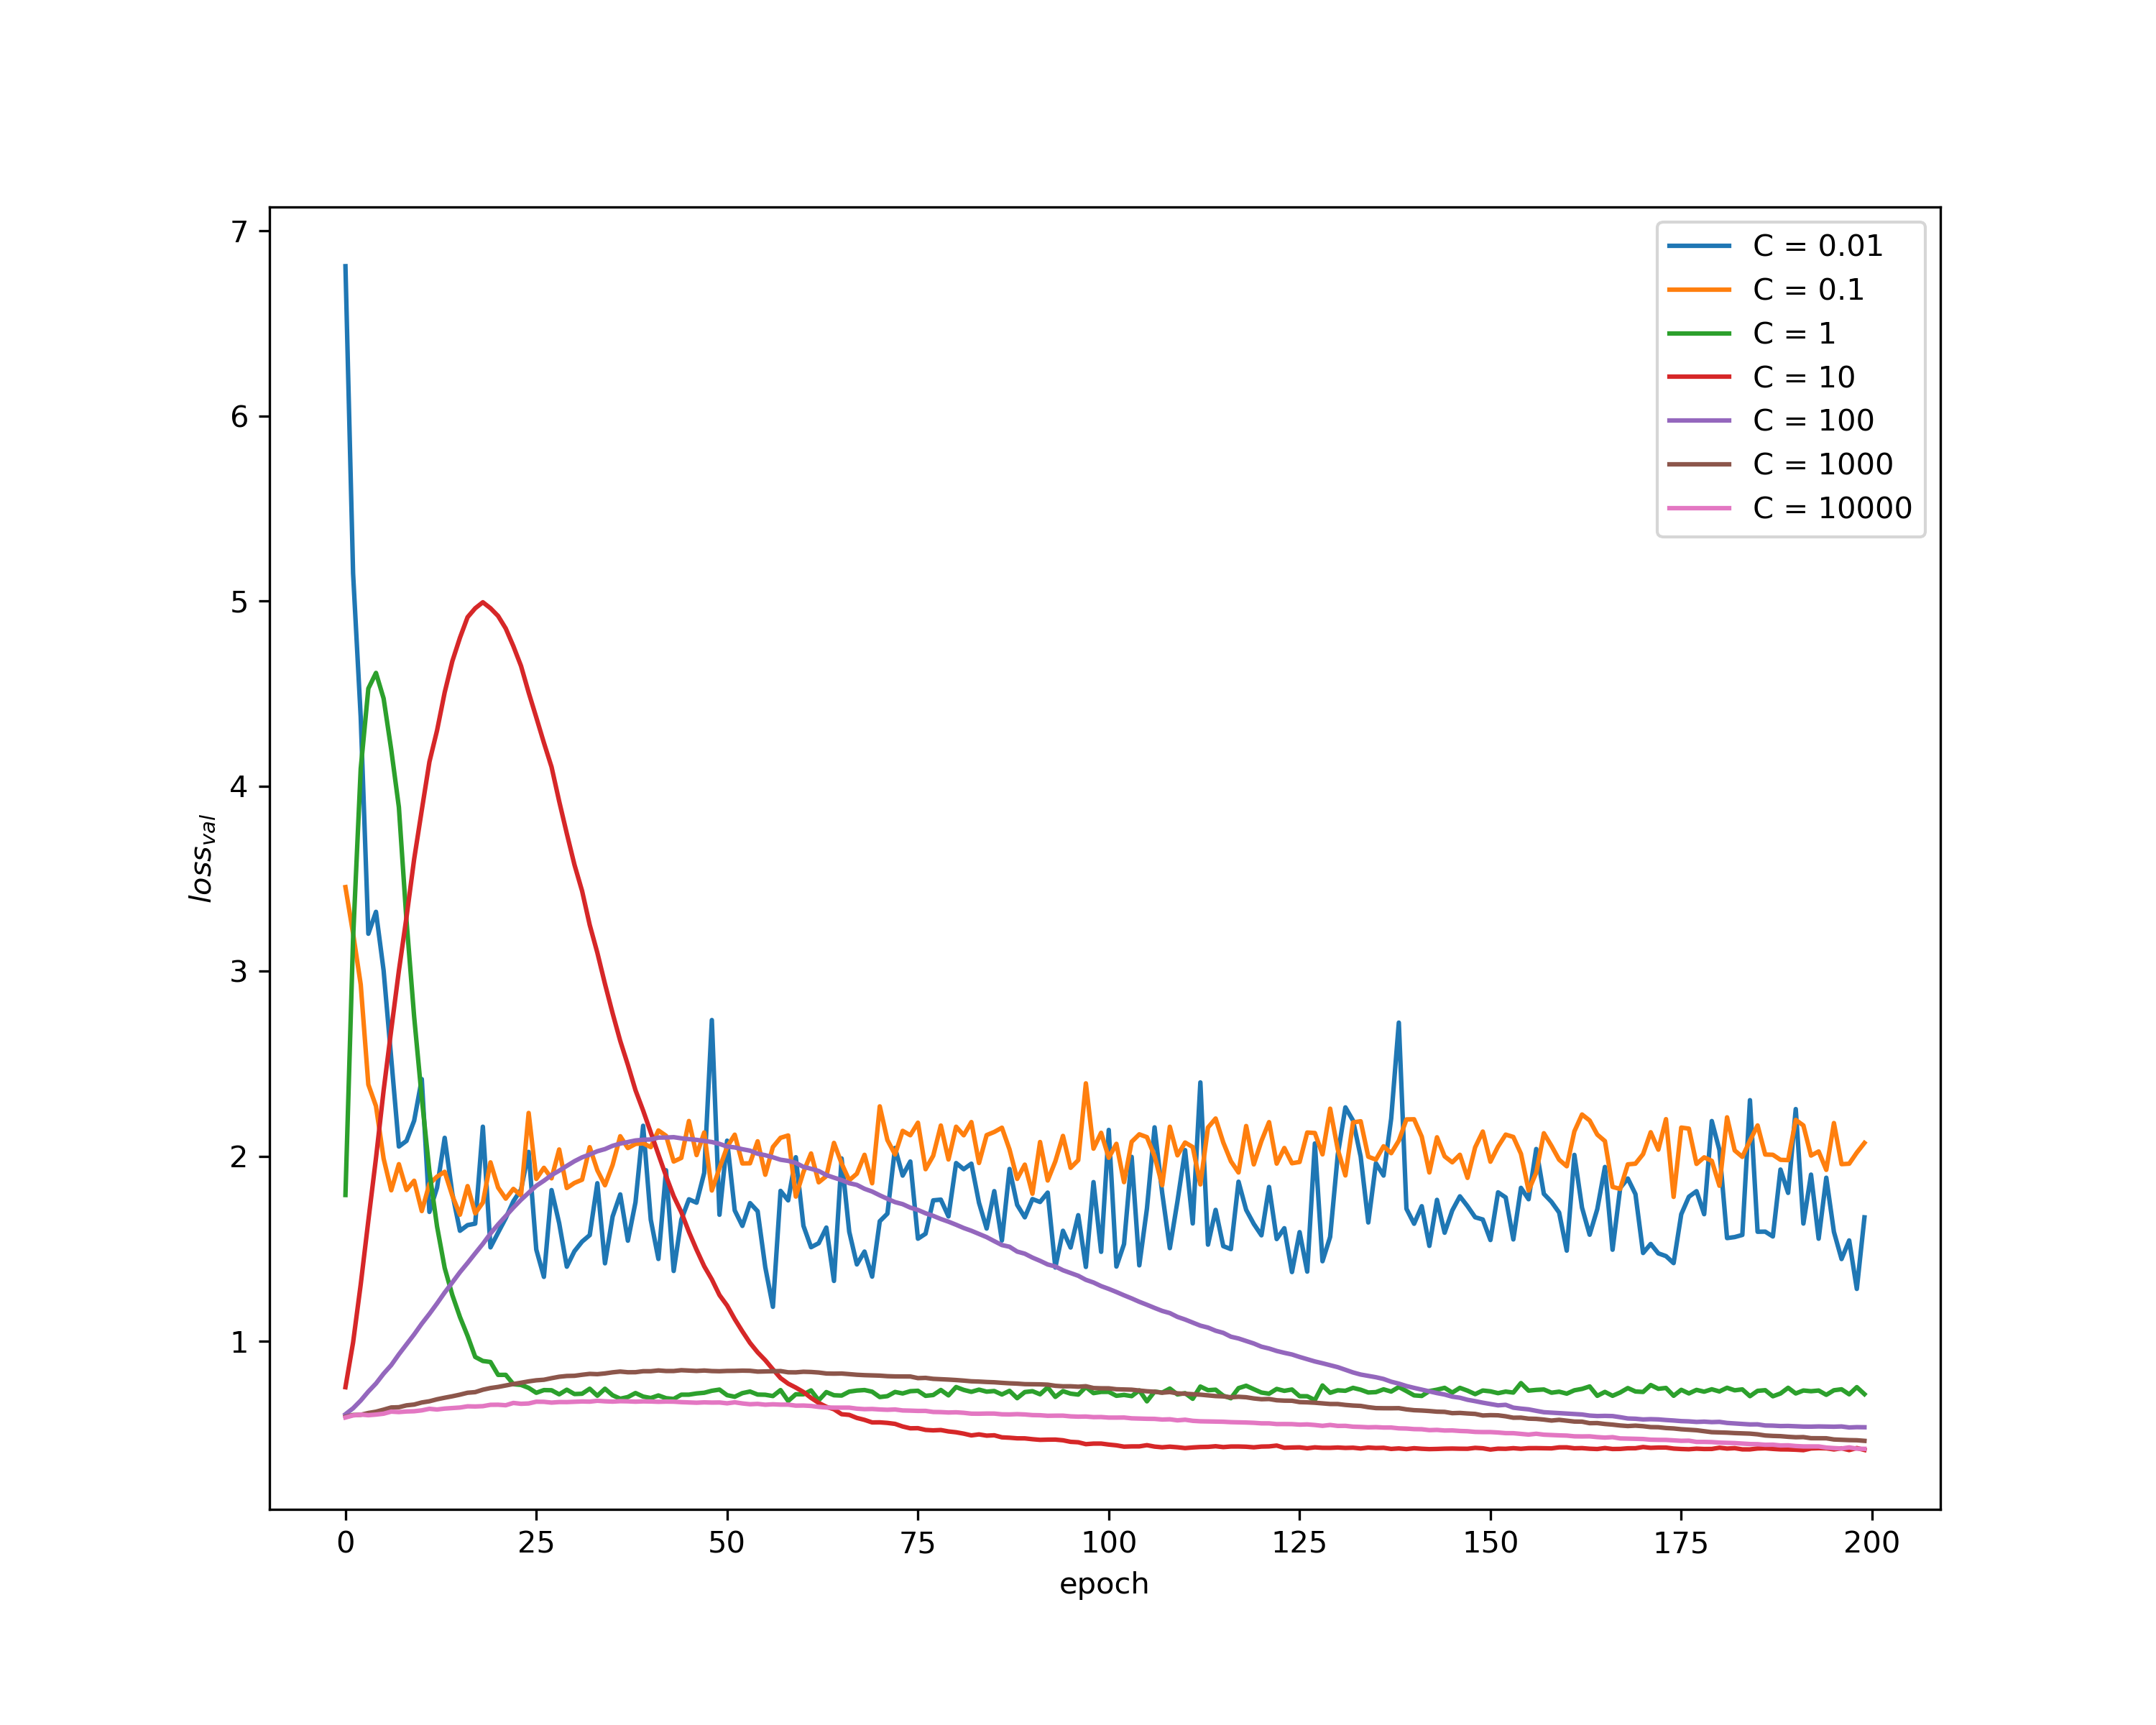
\includegraphics[width=\columnwidth]{c_val_loss}
		% Create a subtitle for the figure.
		\caption{$Loss_{val}$ under different $C$.}
		% Define the label of the figure. It's good to use 'fig:title', so you know that the label belongs to a figure.
		\label{fig:C_loss}
	\end{center}
\end{figure} \par

\begin{figure}[!hbt]
	% Center the figure.
	\begin{center}
		% Include the eps file, scale it such that it's width equals the column width. You can also put width=8cm for example...
		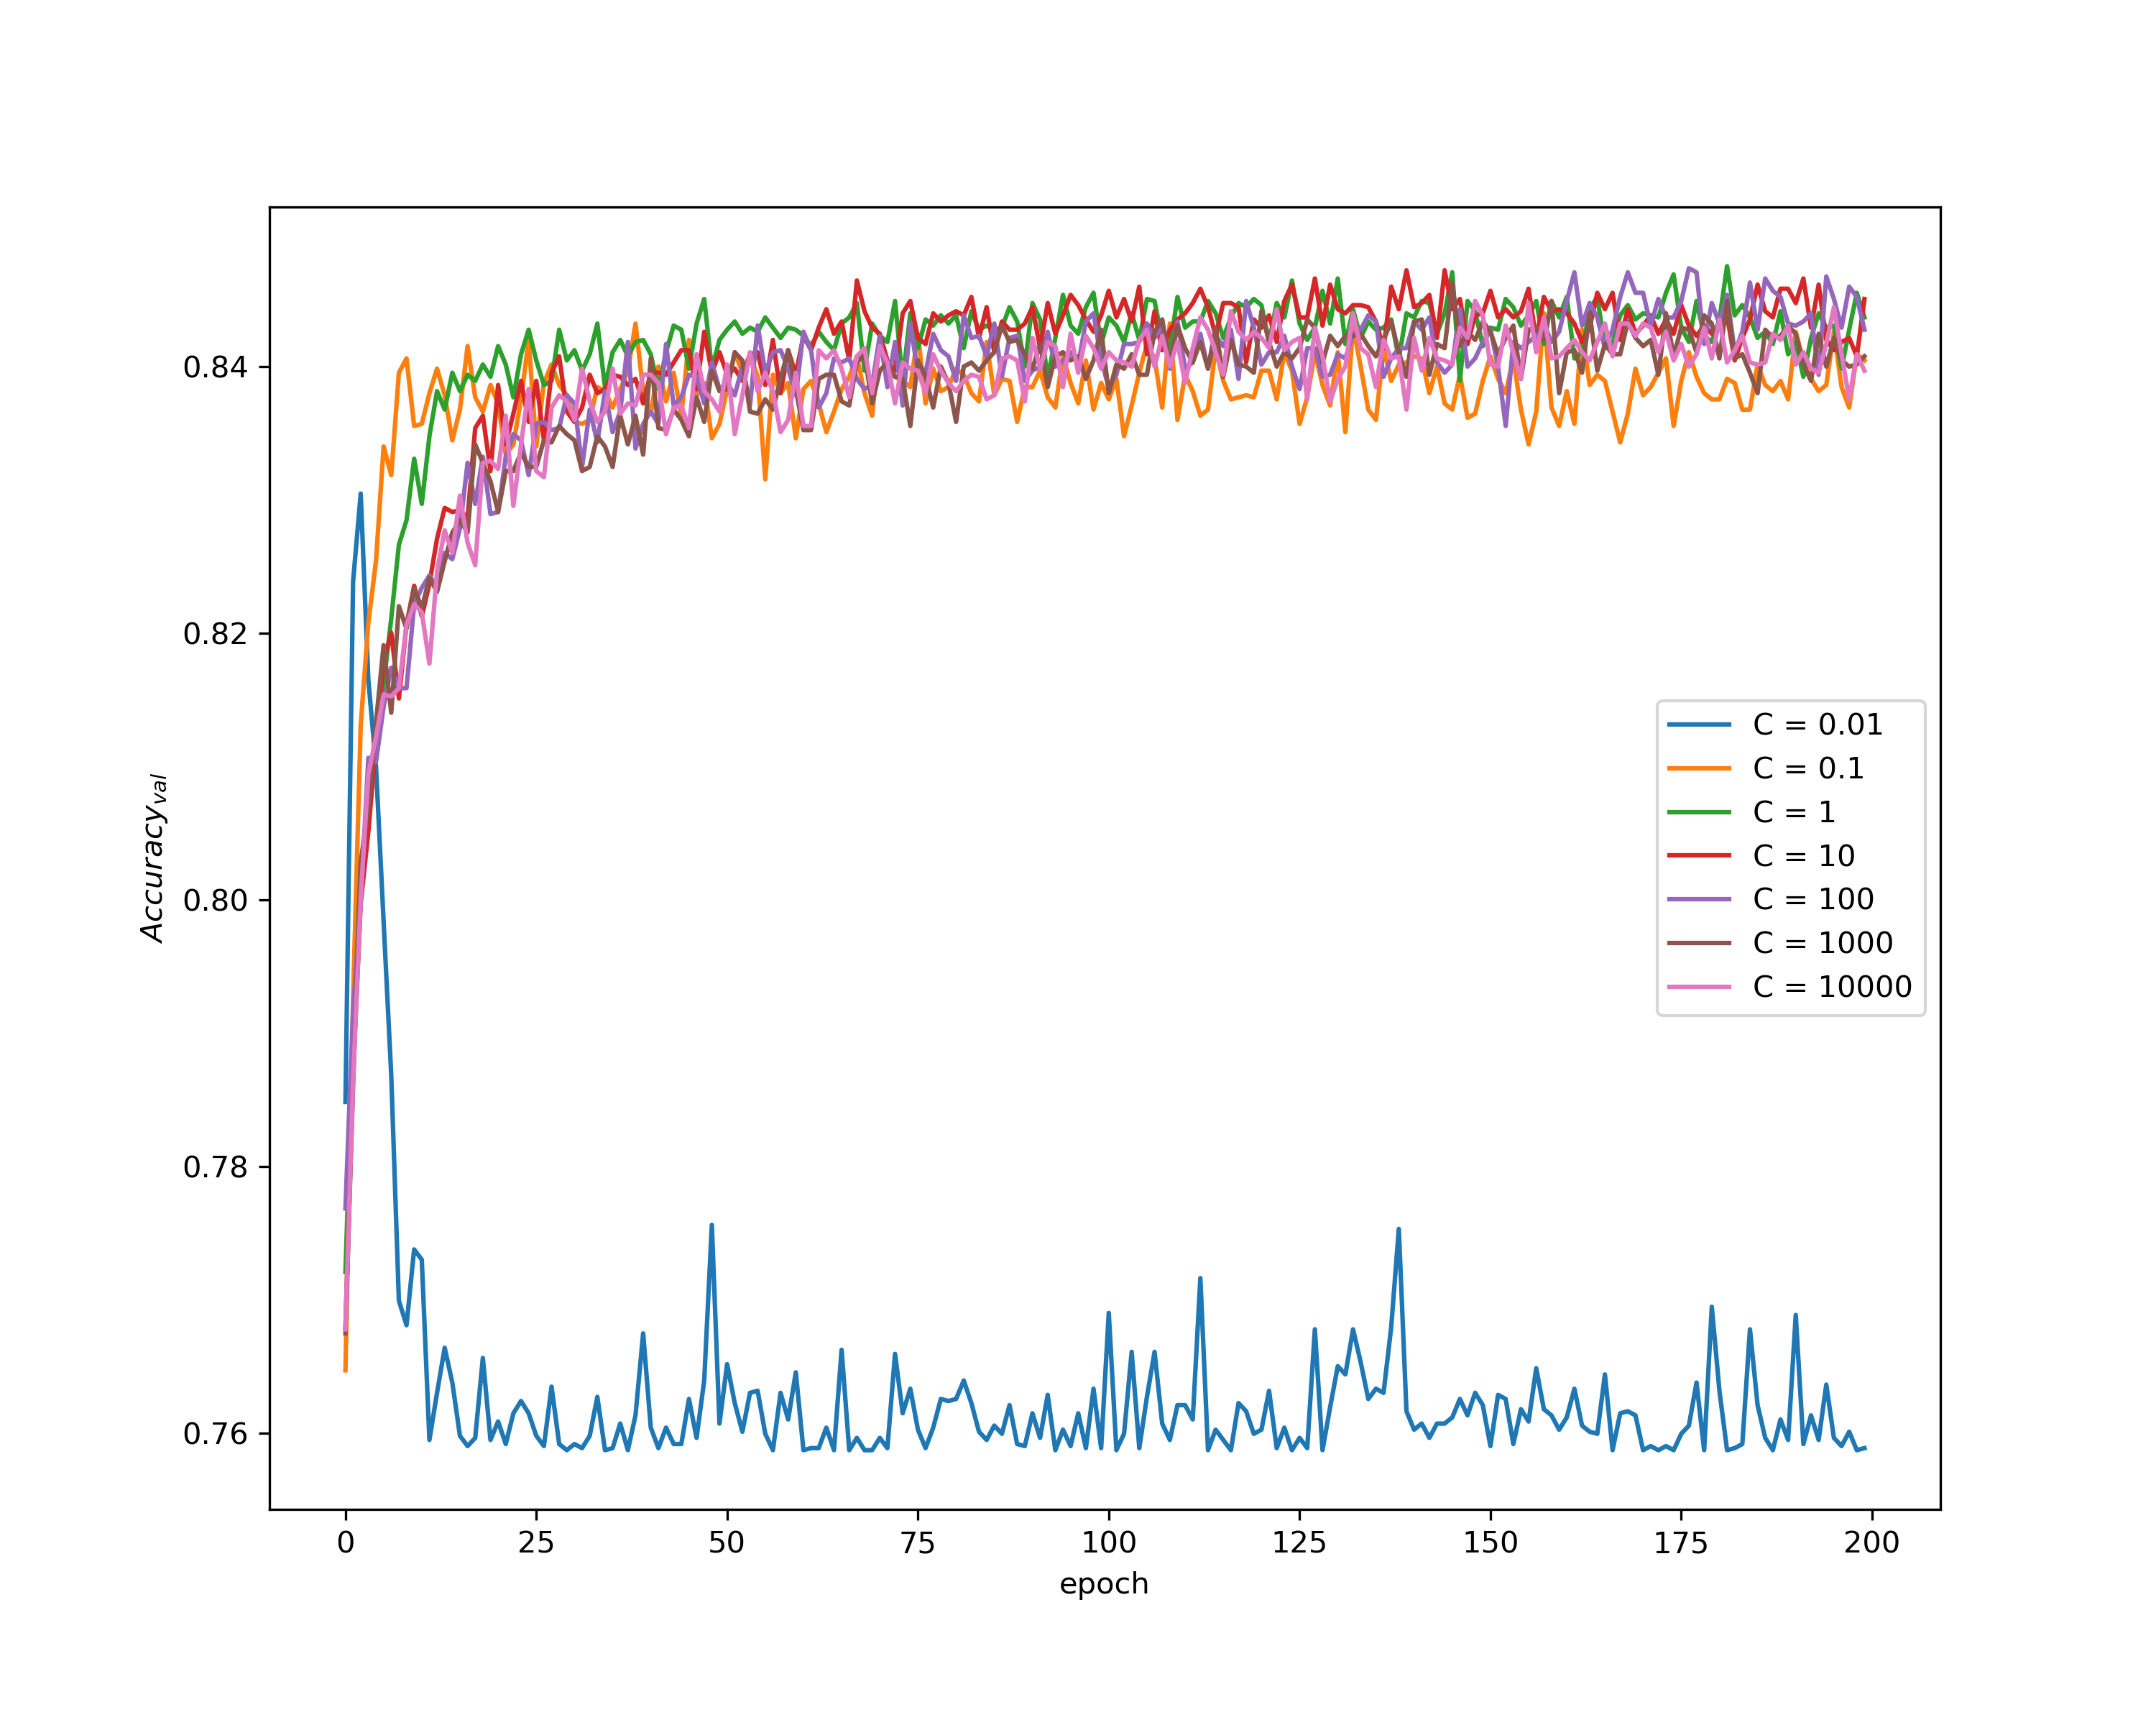
\includegraphics[width=\columnwidth]{c_val_acc}
		% Create a subtitle for the figure.
		\caption{$Accuracy_{val}$ under different $C$.}
		% Define the label of the figure. It's good to use 'fig:title', so you know that the label belongs to a figure.
		\label{fig:C_acc}
	\end{center}
\end{figure} \par

\begin{figure}[!hbt]
	% Center the figure.
	\begin{center}
		% Include the eps file, scale it such that it's width equals the column width. You can also put width=8cm for example...
		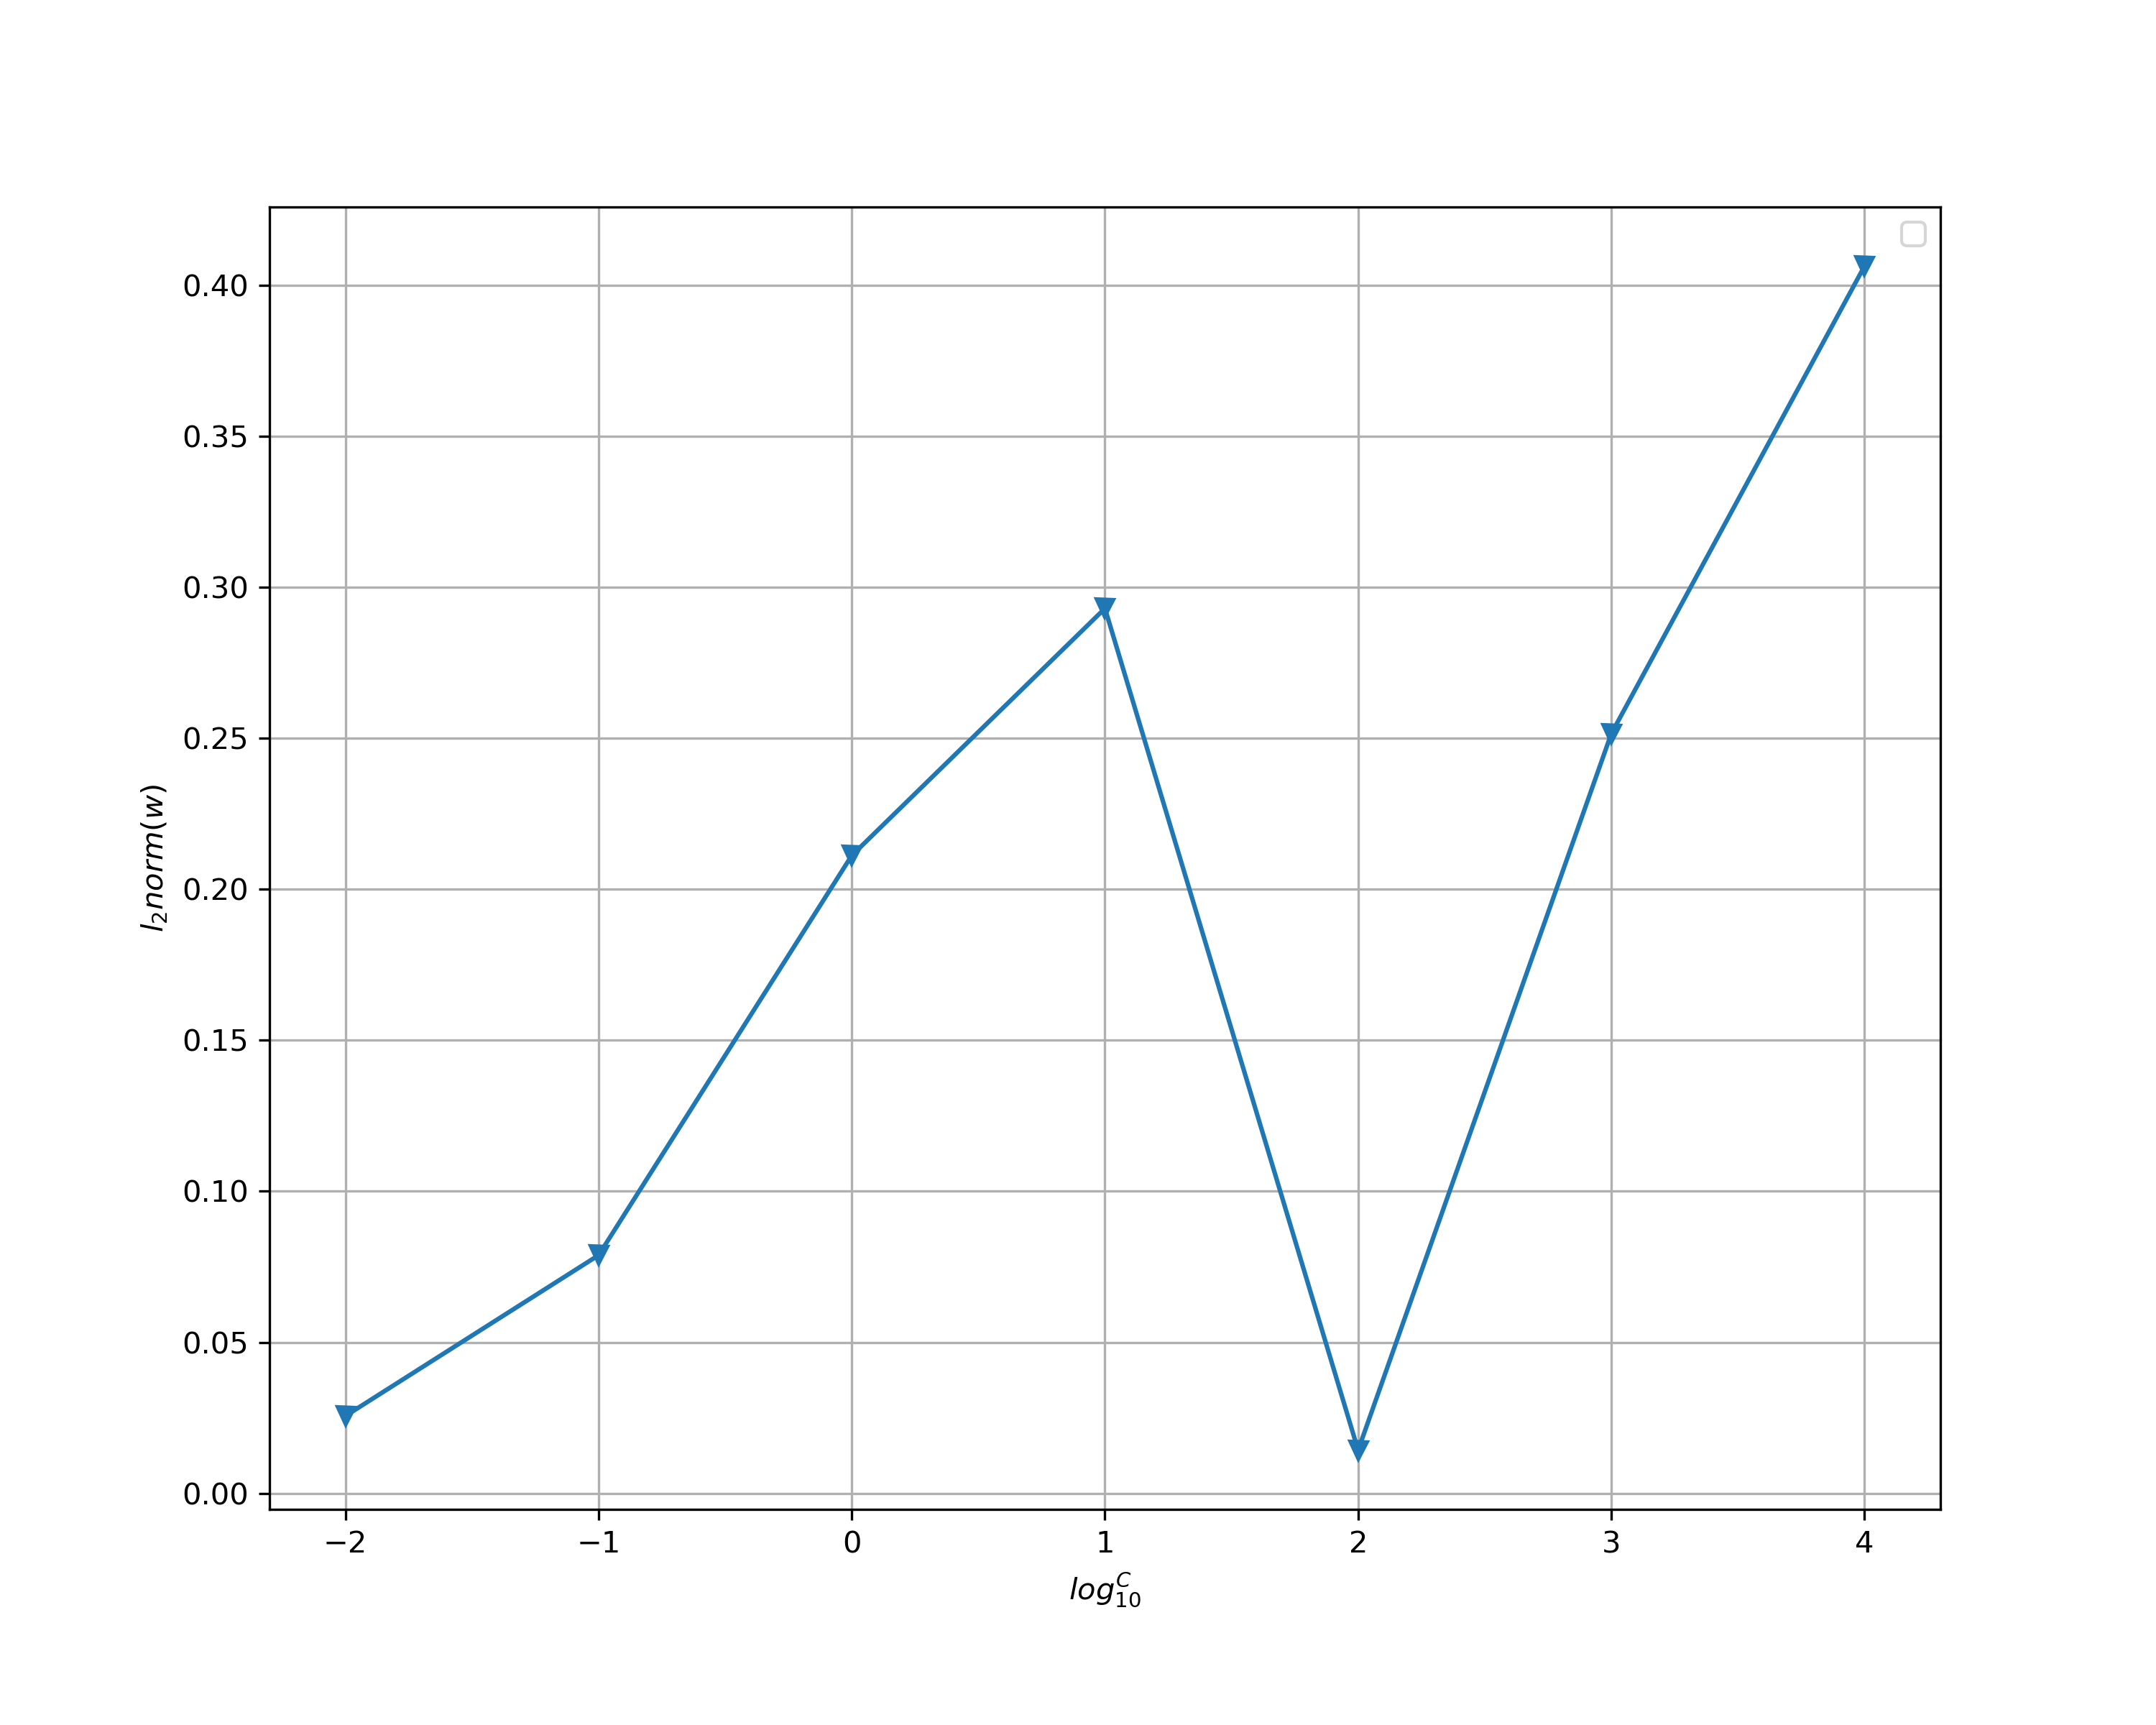
\includegraphics[width=\columnwidth]{c_magnitude}
		% Create a subtitle for the figure.
		\caption{The magnitude of $W$ under different $C$.}
		% Define the label of the figure. It's good to use 'fig:title', so you know that the label belongs to a figure.
		\label{fig:c_mag}
	\end{center}
\end{figure} \par

\begin{table}[!hbt]
	% Center the table
	\begin{center}
		% Title of the table
		\caption{Best Result in Validation set under different C's settings. Best result are in bold.}
		\label{tab:C_performance}
		% Table itself: here we have two columns which are centered and have lines to the left, right and in the middle: |c|c|
		\begin{tabular}{|c|c|c|c|c|c|c|c|}
			% To create a horizontal line, type \hline
			\hline
			% To end a column type &
			% For a linebreak type \\
			$log_{10}^{C}$ & -2 & -1 & 0 & 1 & 2 & 3 & 3 \\
			\hline
			$Accuracy_{val}$   & 84.39 & 84.42 & 84.72 & \textbf{84.75} & 84.73 & 84.56 & 84.49   \\
			\hline
			$Epoch$  & \textbf{2} & 86 & 62 & 138 & 173 & 147 & 145   \\
			\hline
		\end{tabular}
	\end{center}
\end{table} \par


\subsection{Loss function comparision in SVM}
In this section, we conduct experiment on loss function comparision in SVM. Especially, we compare two loss function, hinge loss which is illustrated above And Exponential Loss (EL), where $EL = exp\{-y_i(w^Tx_i + b)\}$. More formaly, $HL(z) = max(0, 1 - z)$ and $EL(z) = exp^{-z}$. Fig~\ref{fig:loss_fn} shows that HL and EL both have one advantage and one disadvantage. HL is stable when z is very mall, however EL become very large, which will lead to numeric unstable. EL is derivable every but HL is not derivable when $z = 1$. We use SGD as optimizer with learning rate 0.001, set epoch to 200, batch size to 64 and C to 10.\par
From Fig~\ref{fig:l_val_loss} and Fig~\ref{fig:l_val_acc}, we can see that the performance of HL is superior. EL has numeric unstablity problem during gradient descent process. \par
\begin{figure}[!hbt]
	% Center the figure.
	\begin{center}
		% Include the eps file, scale it such that it's width equals the column width. You can also put width=8cm for example...
		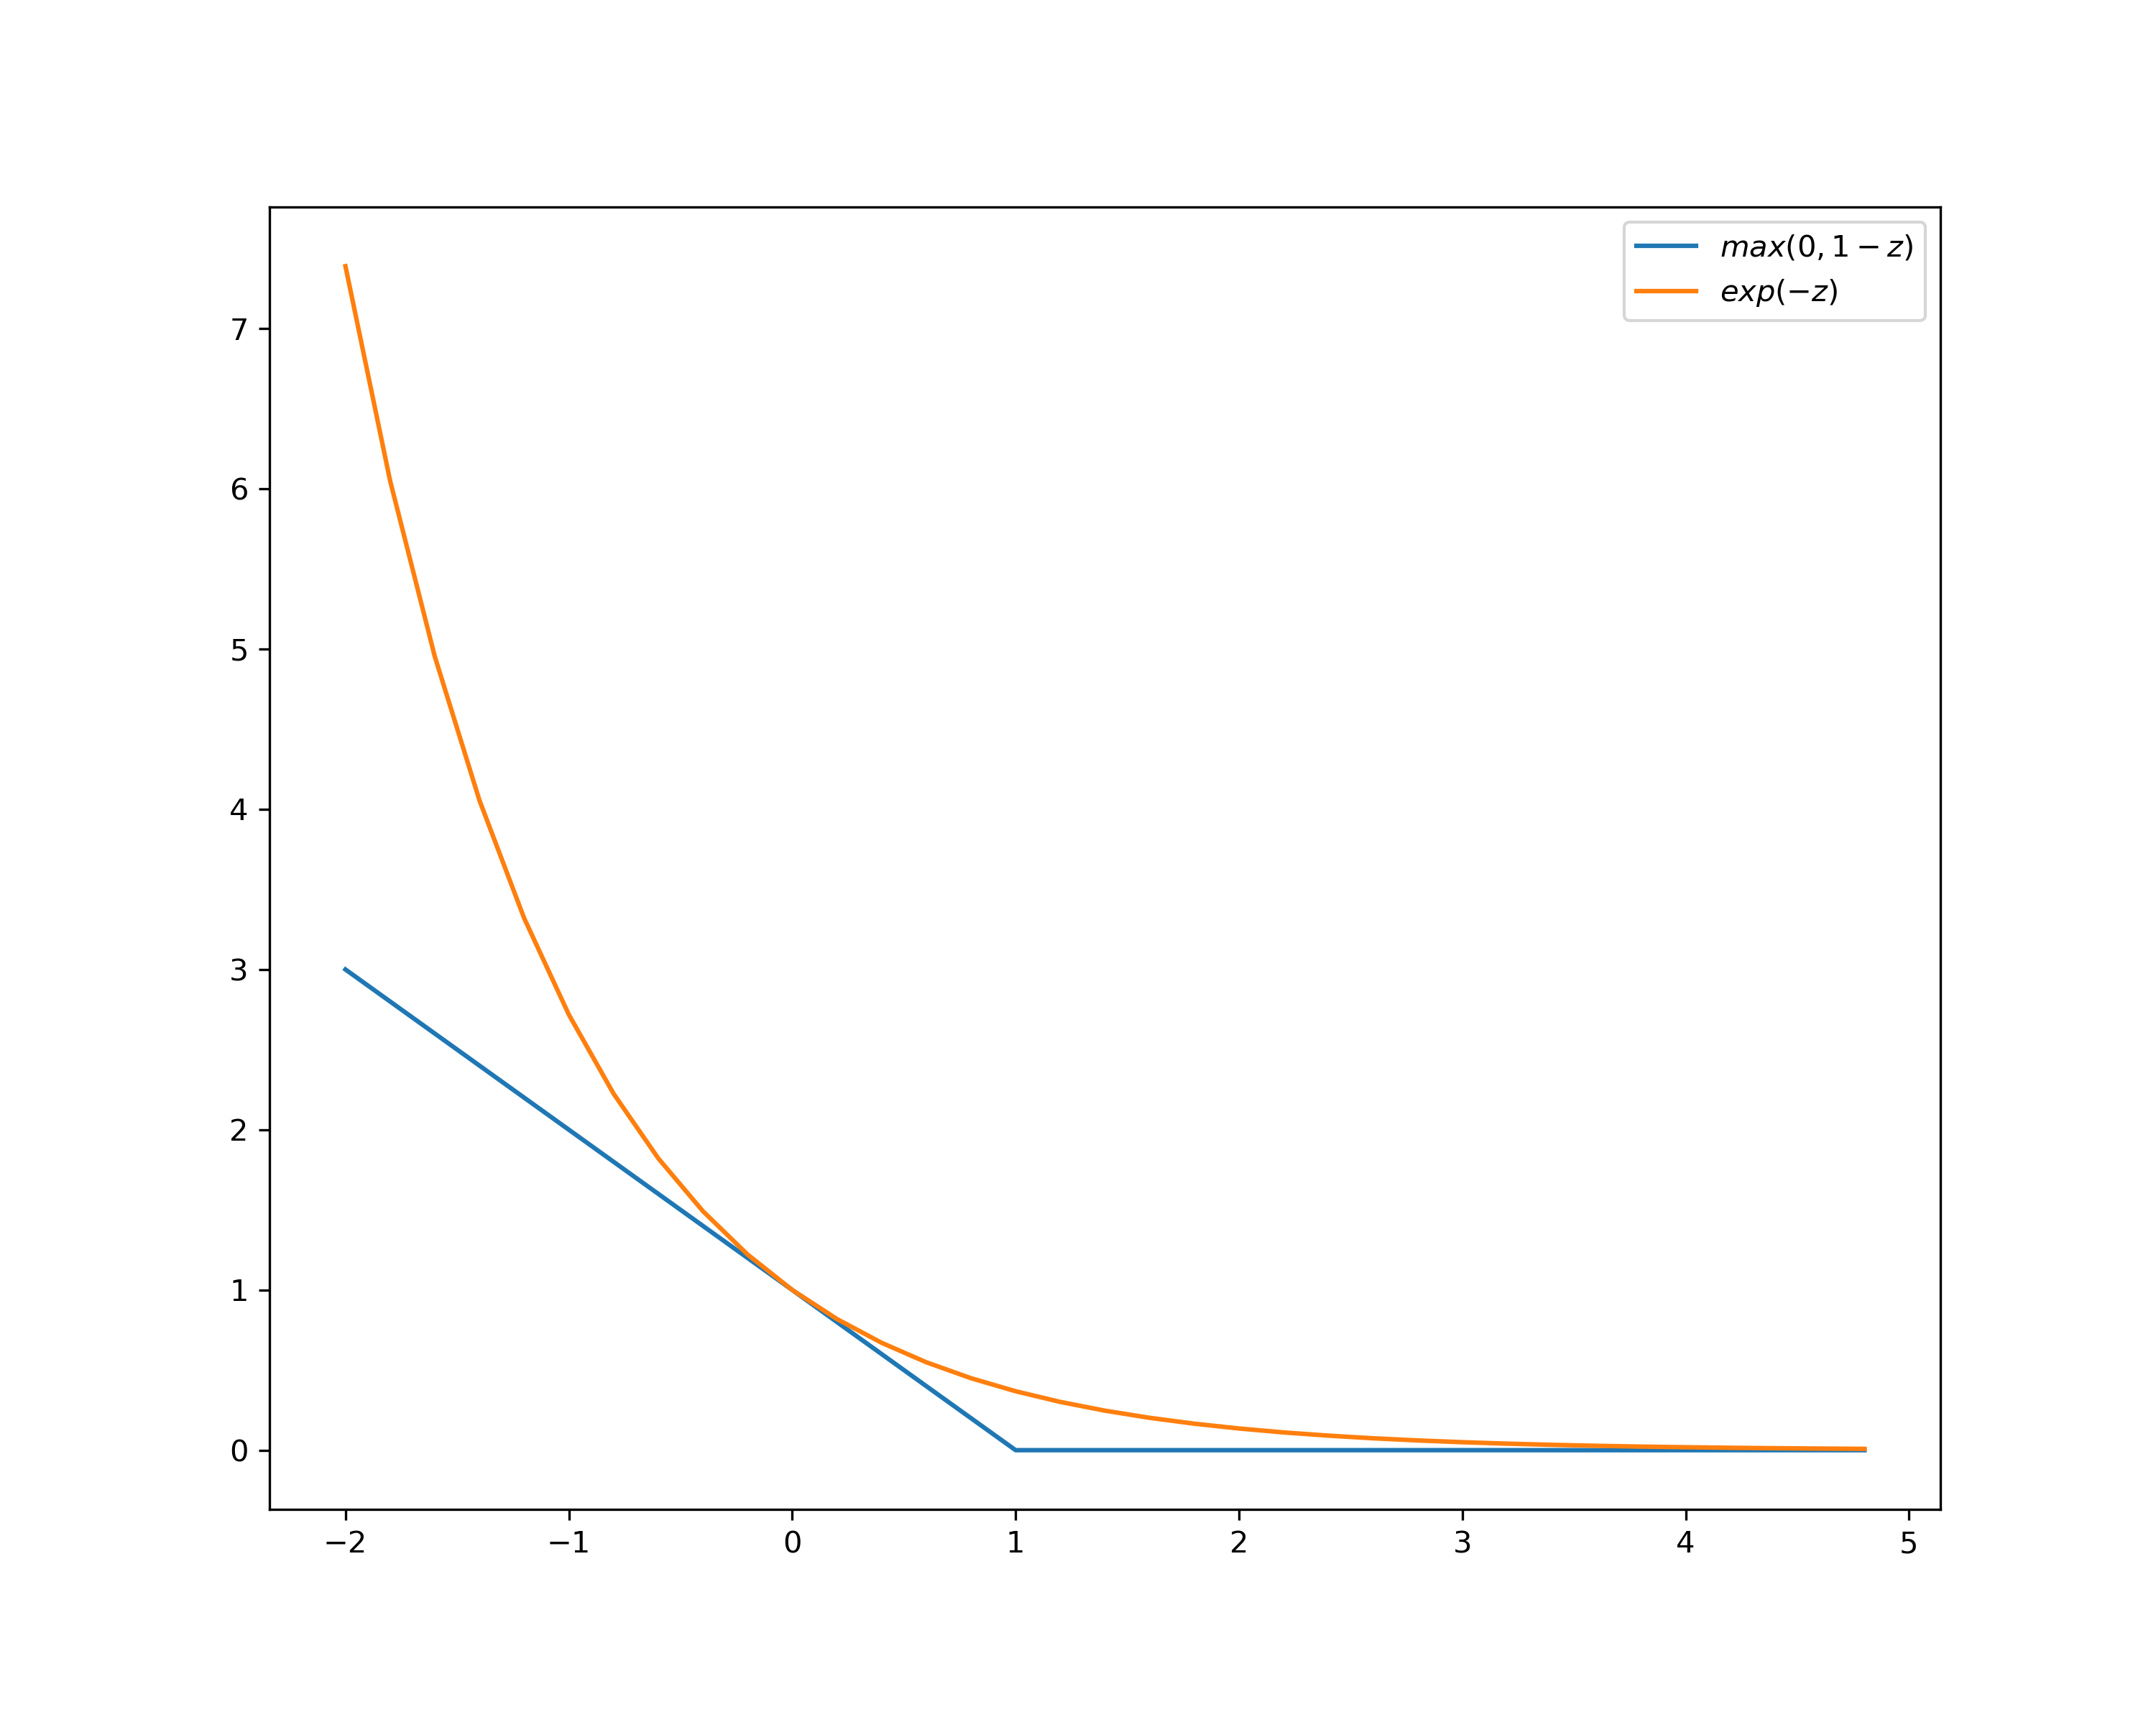
\includegraphics[width=\columnwidth]{loss_fn}
		% Create a subtitle for the figure.
		\caption{The plot of HL and EL.}
		% Define the label of the figure. It's good to use 'fig:title', so you know that the label belongs to a figure.
		\label{fig:loss_fn}
	\end{center}
\end{figure} \par

\begin{figure}[!hbt]
	% Center the figure.
	\begin{center}
		% Include the eps file, scale it such that it's width equals the column width. You can also put width=8cm for example...
		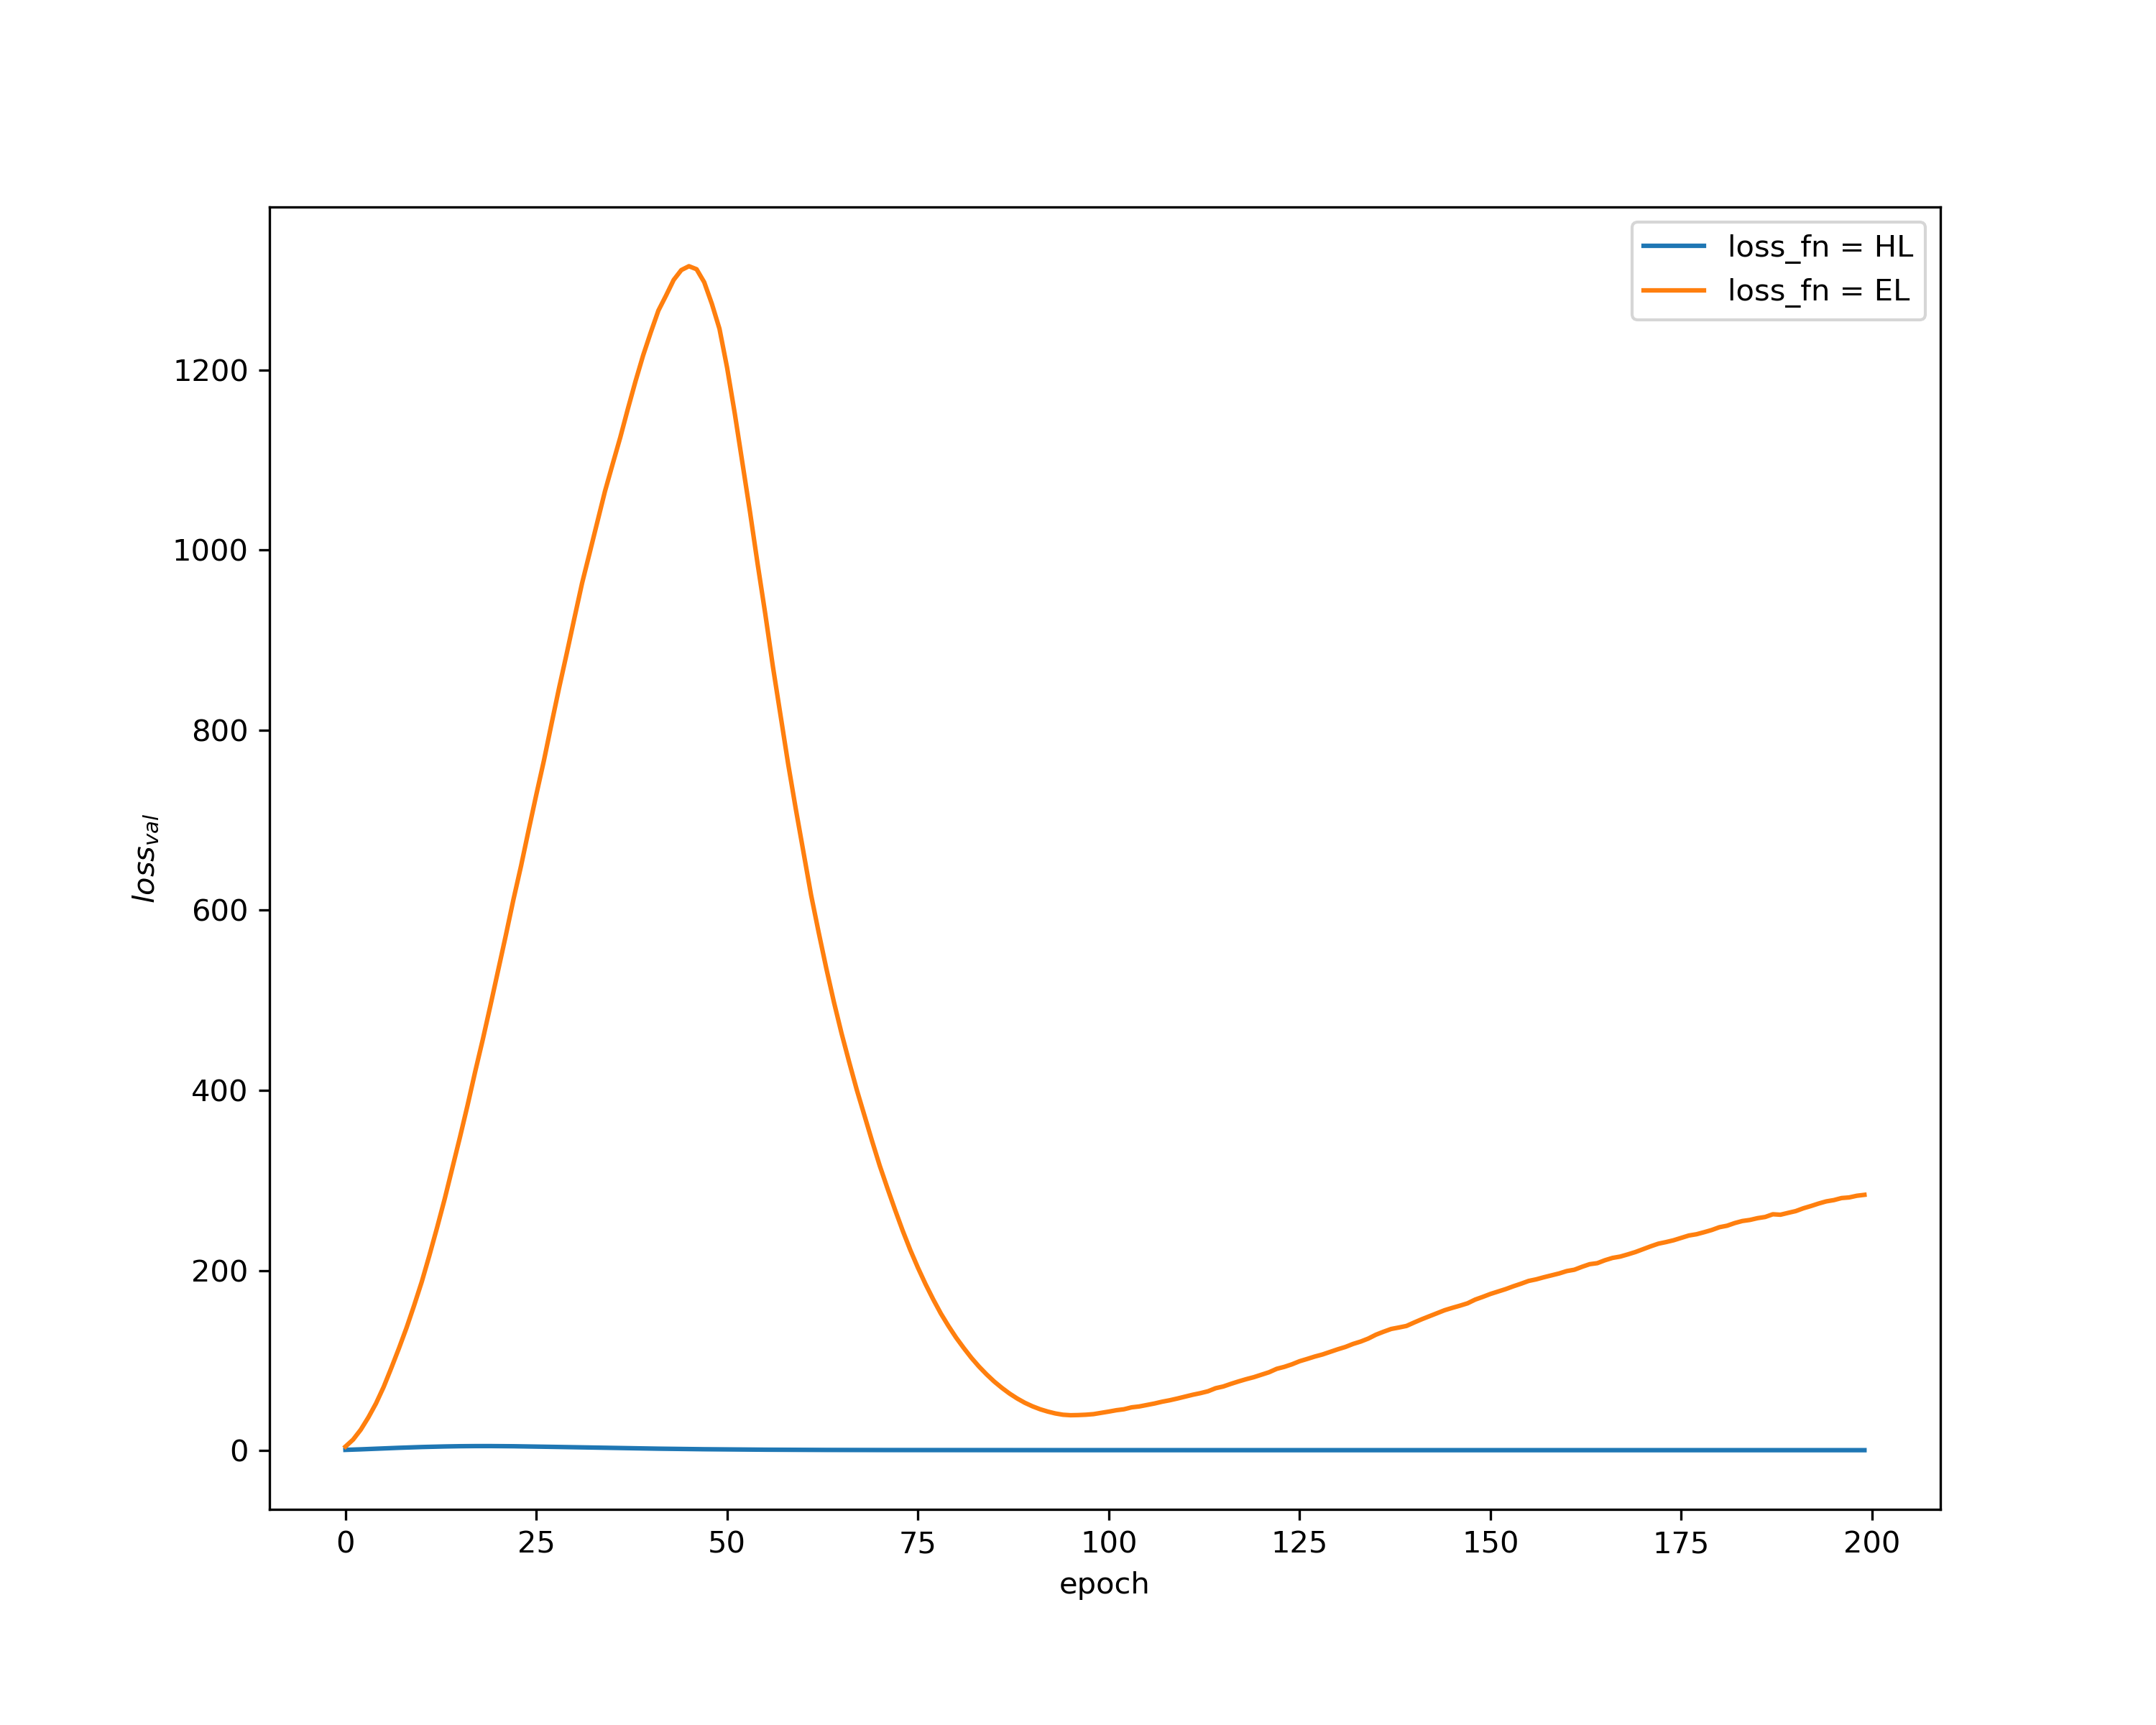
\includegraphics[width=\columnwidth]{l_val_loss}
		% Create a subtitle for the figure.
		\caption{$loss_{val}$ under different loss function.}
		% Define the label of the figure. It's good to use 'fig:title', so you know that the label belongs to a figure.
		\label{fig:l_val_loss}
	\end{center}
\end{figure} \par

\begin{figure}[!hbt]
	% Center the figure.
	\begin{center}
		% Include the eps file, scale it such that it's width equals the column width. You can also put width=8cm for example...
		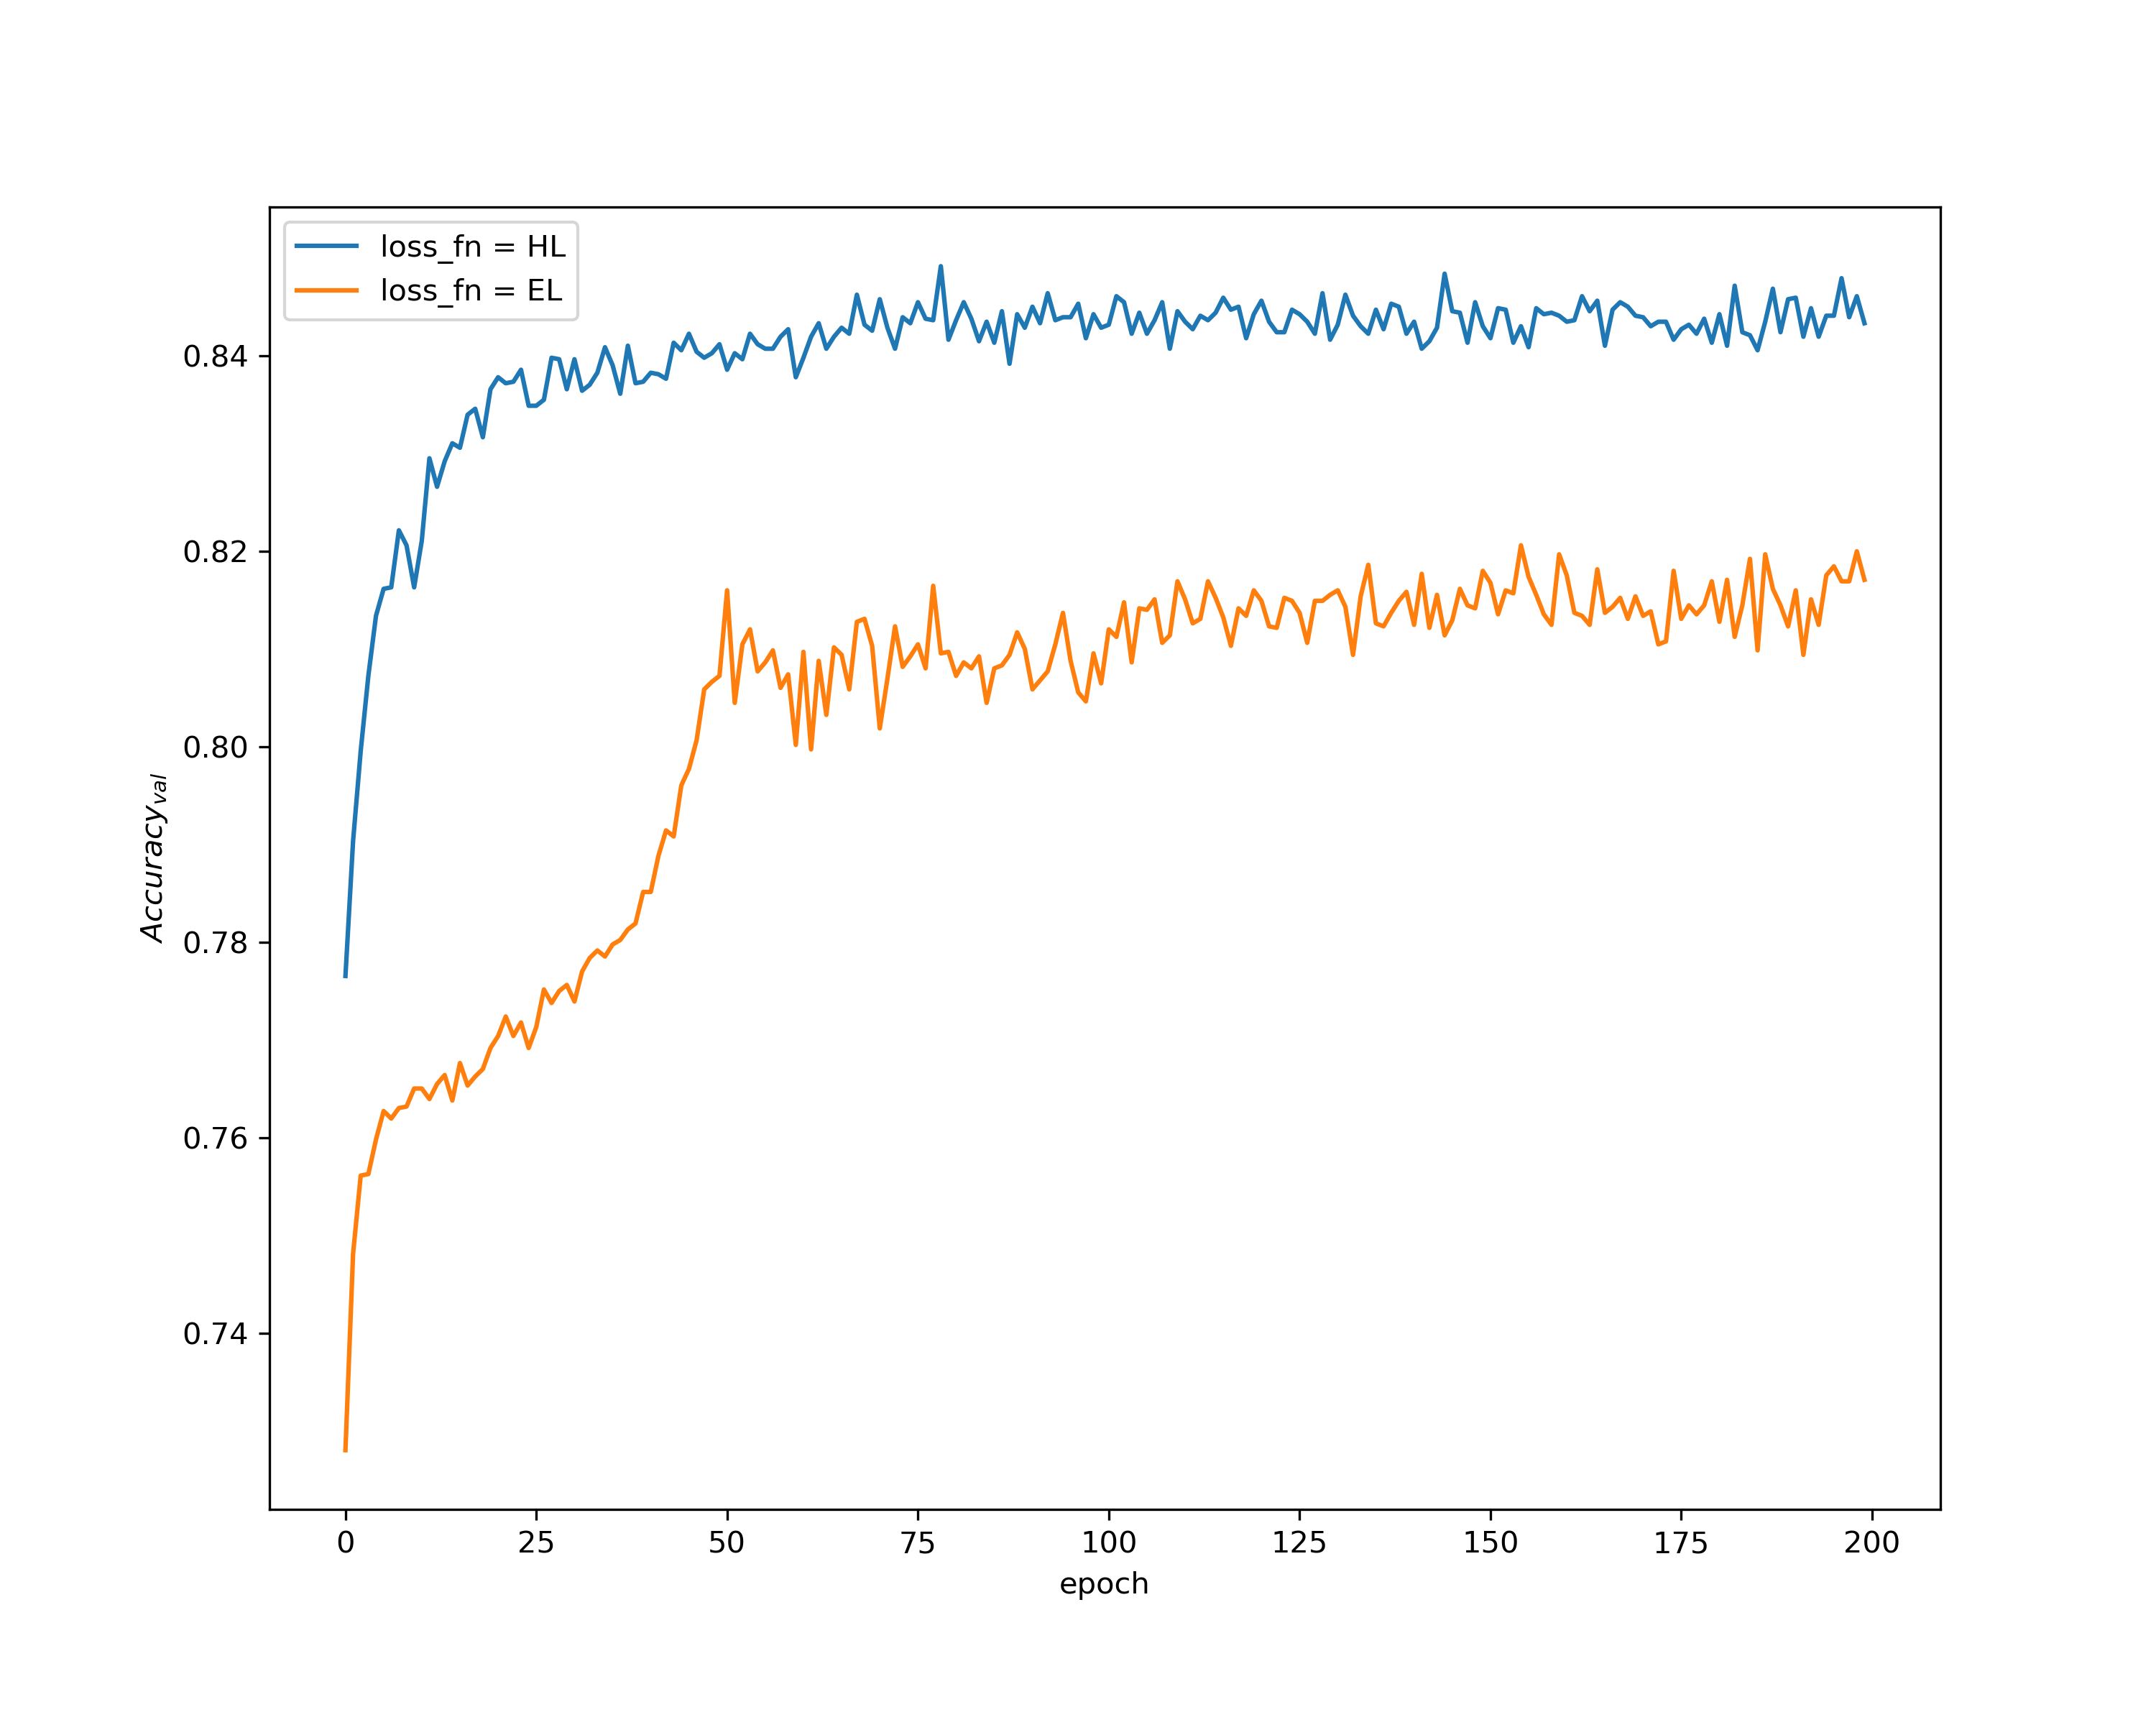
\includegraphics[width=\columnwidth]{l_val_acc}
		% Create a subtitle for the figure.
		\caption{$Accuracy_{val}$ under different loss function.}
		% Define the label of the figure. It's good to use 'fig:title', so you know that the label belongs to a figure.
		\label{fig:l_val_acc}
	\end{center}
\end{figure} \par

\subsection{Initilizer comparision in both LR and SVM}
In this section, we compare the performance of LR and SVM under different initilizers. We explore over ones, zeros, xavier uniform and random initializer. Ones initilizers makes the initial $w$ to all one and Zeros initilizers makes the initial $w$ to all zero. Xavier uniform initializer uniformally initial $w$, but bounded to interval $[-n, n]$, where $n$ is $W$'s dimension. Random initializer initial $w$ from standard normal distribution. We use SGD as optimizer with learning rate 0.001, set epoch to 200, batch size to 64 and C to 10 in SVM. We use HL as SVM's loss function and BCE as LR's loss function.\par
From Fig~\ref{fig:lr_init_val_loss} and Fig~\ref{fig:lr_init_val_acc}, we can see that LR's performance is affected by the initilizer. Typically Ones initilizer brings the worst performance and Xavier uniform initializer bring the best performance. \par
From Fig~\ref{fig:svm_init_val_loss} and Fig~\ref{fig:svm_init_val_acc}, we can see that SVM is very robust to the initilizer, different initilizer didn't disturb the performance. \par

\begin{figure}[!hbt]
	% Center the figure.
	\begin{center}
		% Include the eps file, scale it such that it's width equals the column width. You can also put width=8cm for example...
		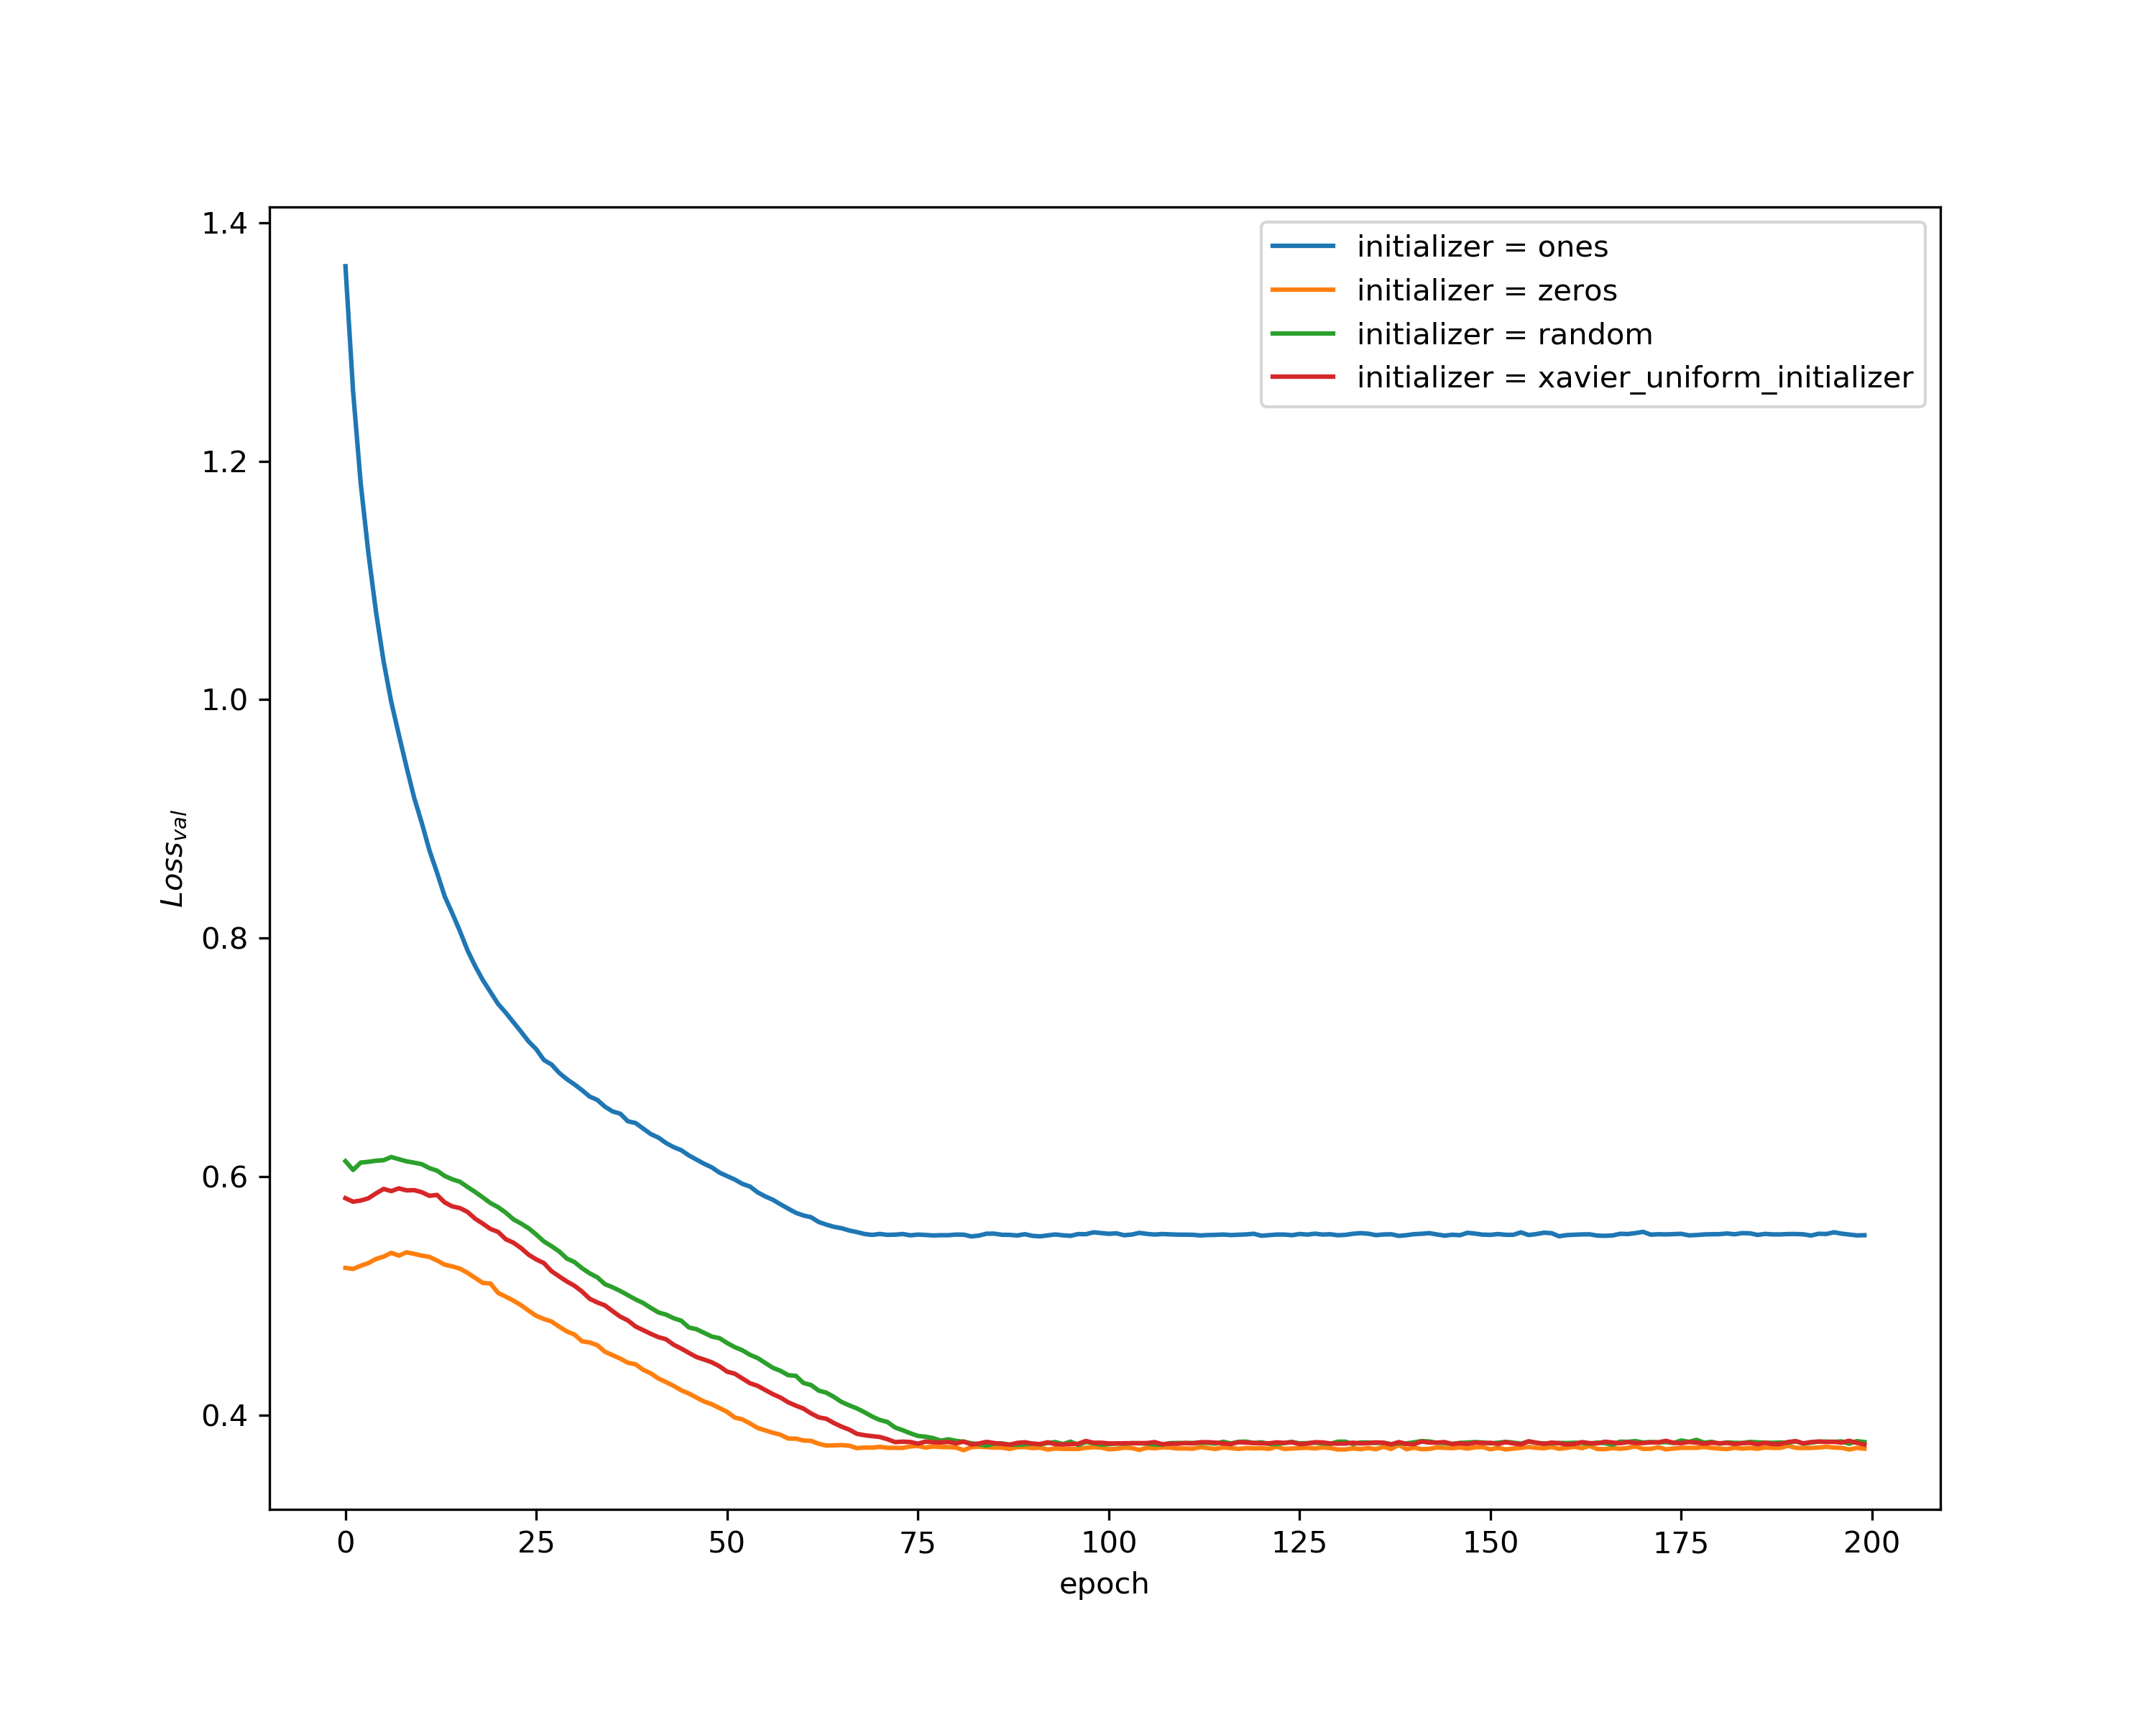
\includegraphics[width=\columnwidth]{lr_init_val_loss}
		% Create a subtitle for the figure.
		\caption{LR's $BCE_{val}$ under different initilizer.}
		% Define the label of the figure. It's good to use 'fig:title', so you know that the label belongs to a figure.
		\label{fig:lr_init_val_loss}
	\end{center}
\end{figure} \par

\begin{figure}[!hbt]
	% Center the figure.
	\begin{center}
		% Include the eps file, scale it such that it's width equals the column width. You can also put width=8cm for example...
		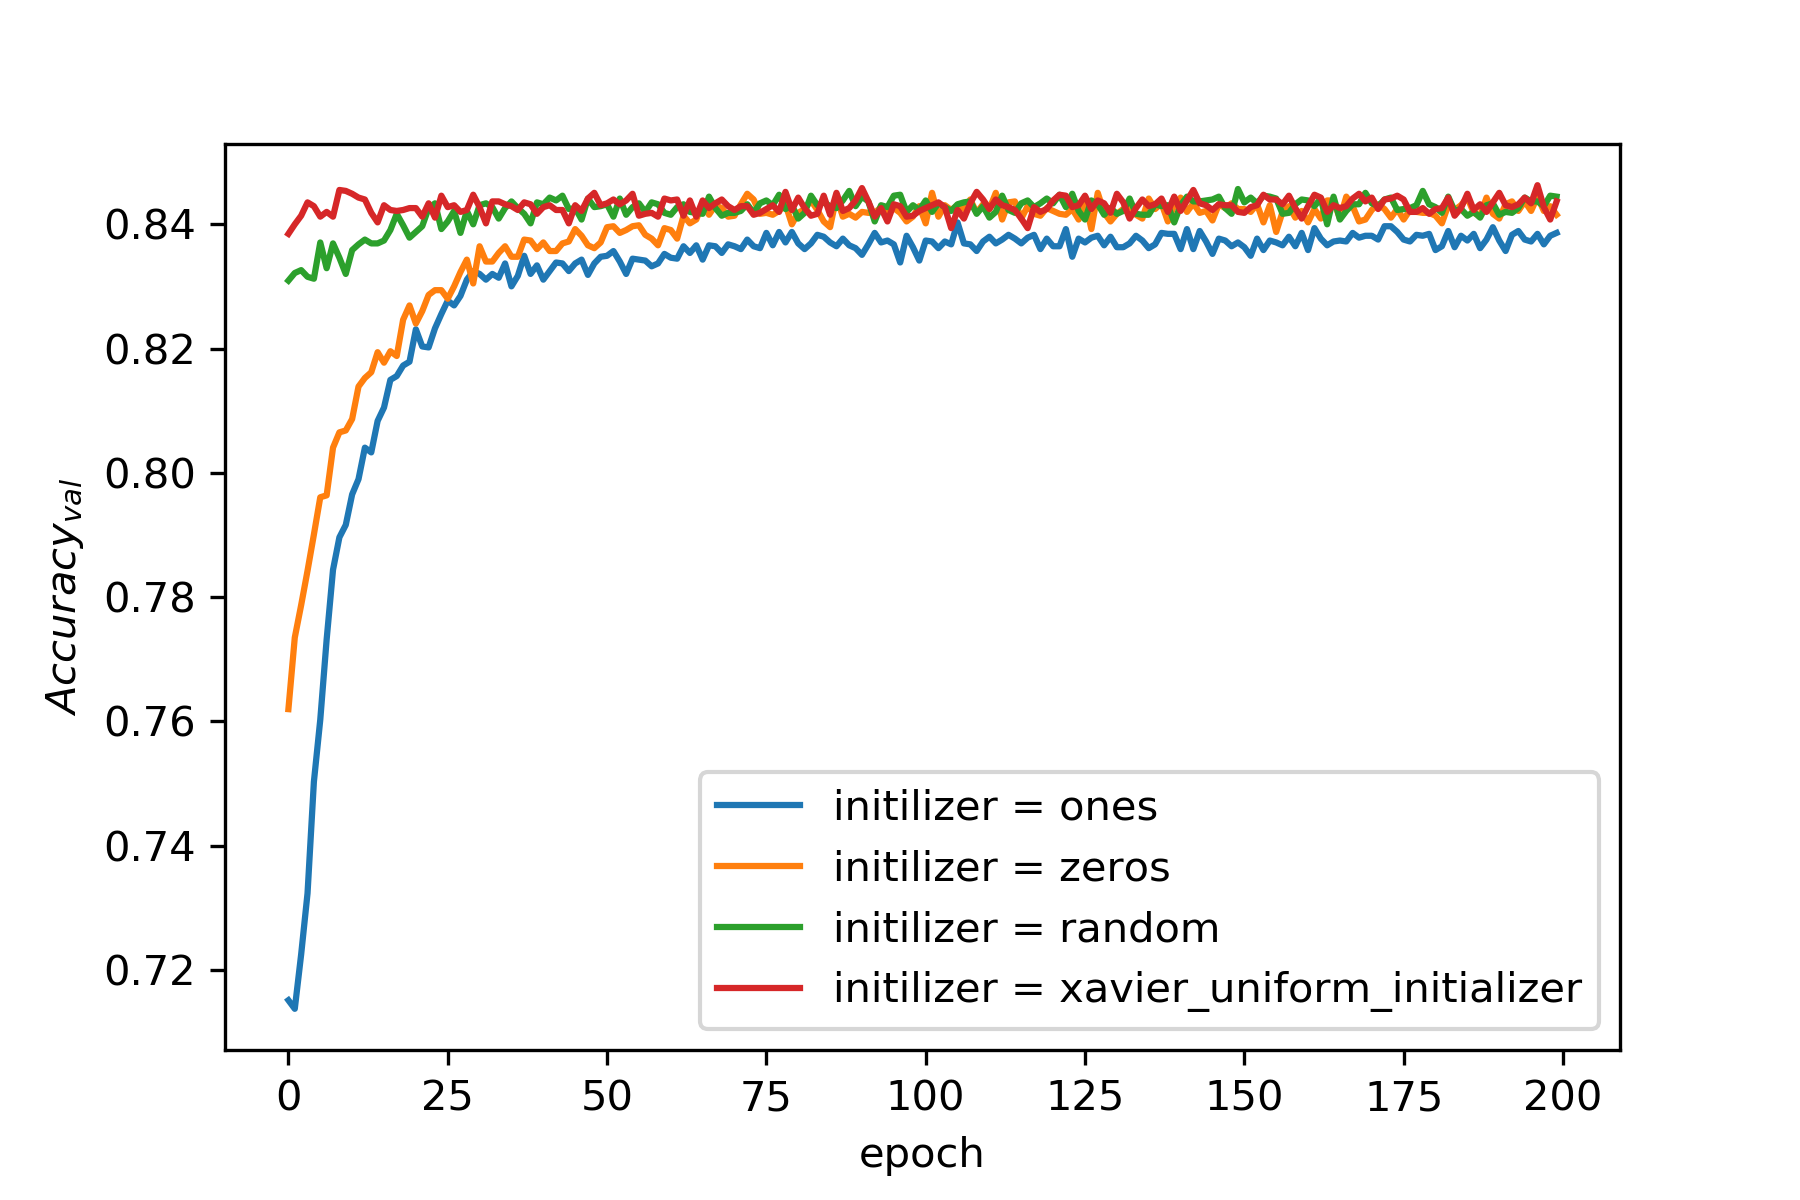
\includegraphics[width=\columnwidth]{lr_init_val_acc}
		% Create a subtitle for the figure.
		\caption{LR's $Accuracy_{val}$ under different initilizer.}
		% Define the label of the figure. It's good to use 'fig:title', so you know that the label belongs to a figure.
		\label{fig:lr_init_val_acc}
	\end{center}
\end{figure} \par

\begin{figure}[!hbt]
	% Center the figure.
	\begin{center}
		% Include the eps file, scale it such that it's width equals the column width. You can also put width=8cm for example...
		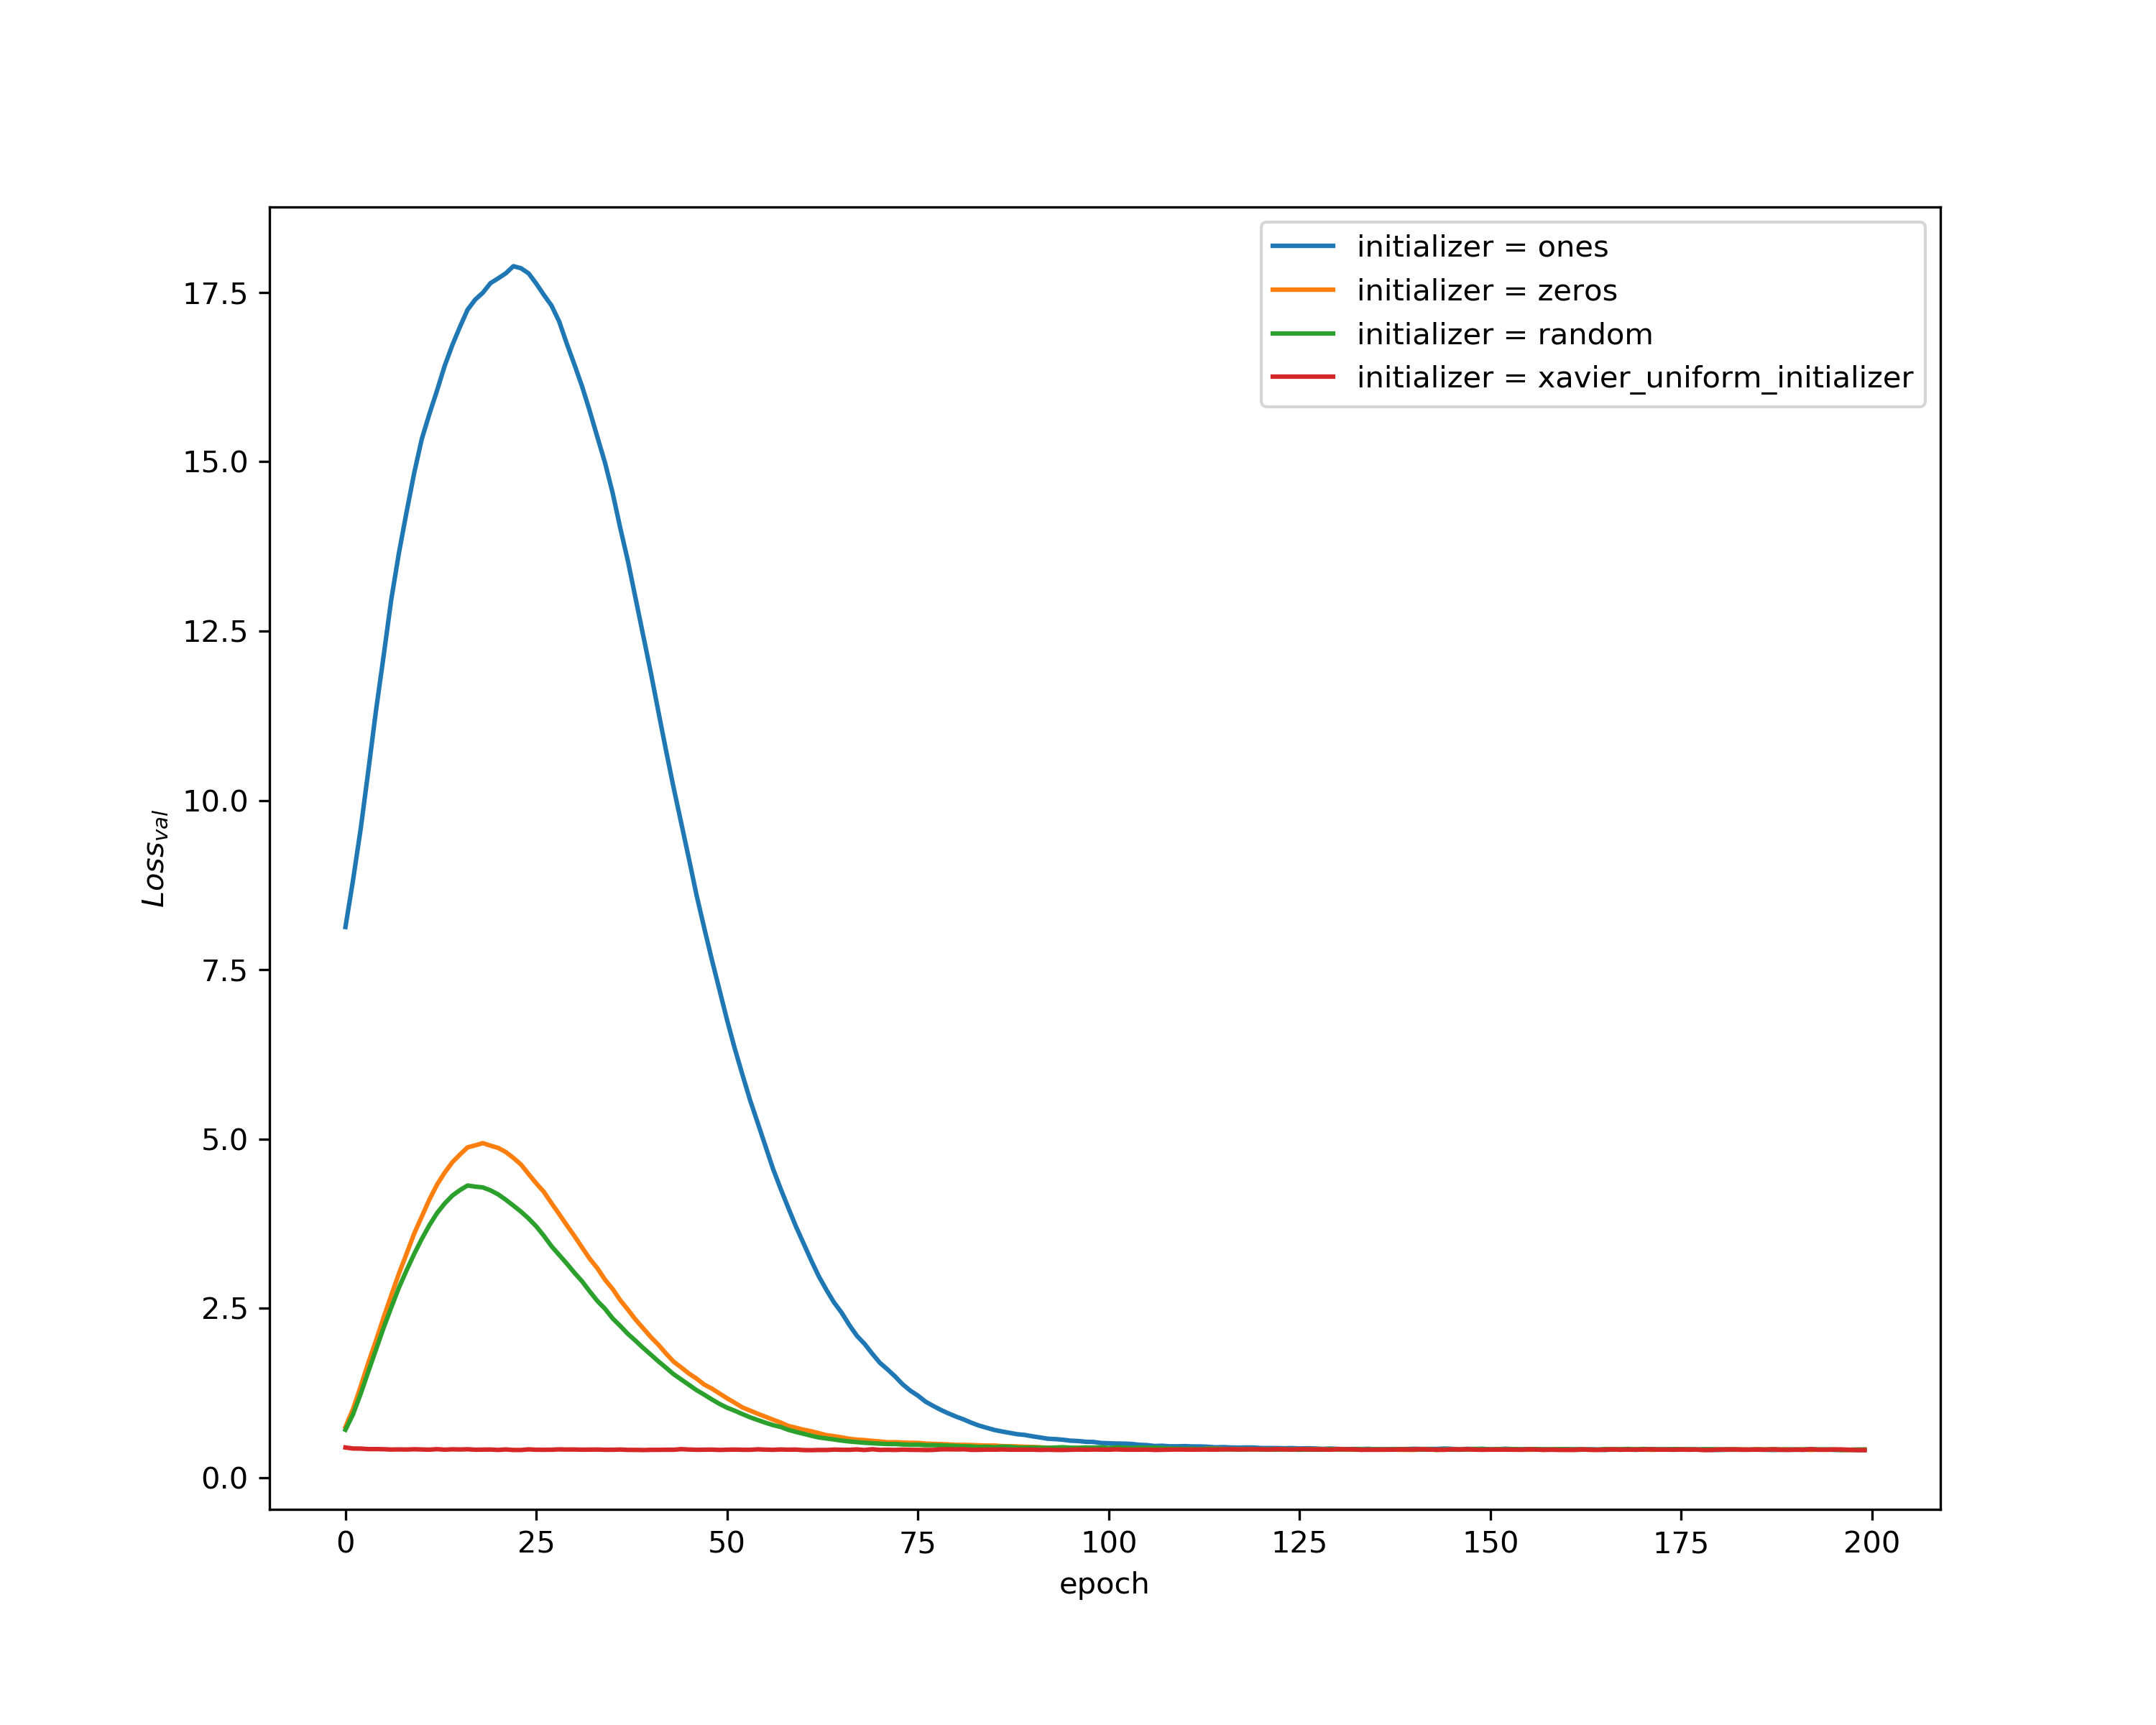
\includegraphics[width=\columnwidth]{svm_init_val_loss}
		% Create a subtitle for the figure.
		\caption{SVM's $HL_{val}$ under different initilizer.}
		% Define the label of the figure. It's good to use 'fig:title', so you know that the label belongs to a figure.
		\label{fig:svm_init_val_loss}
	\end{center}
\end{figure} \par

\begin{figure}[!hbt]
	% Center the figure.
	\begin{center}
		% Include the eps file, scale it such that it's width equals the column width. You can also put width=8cm for example...
		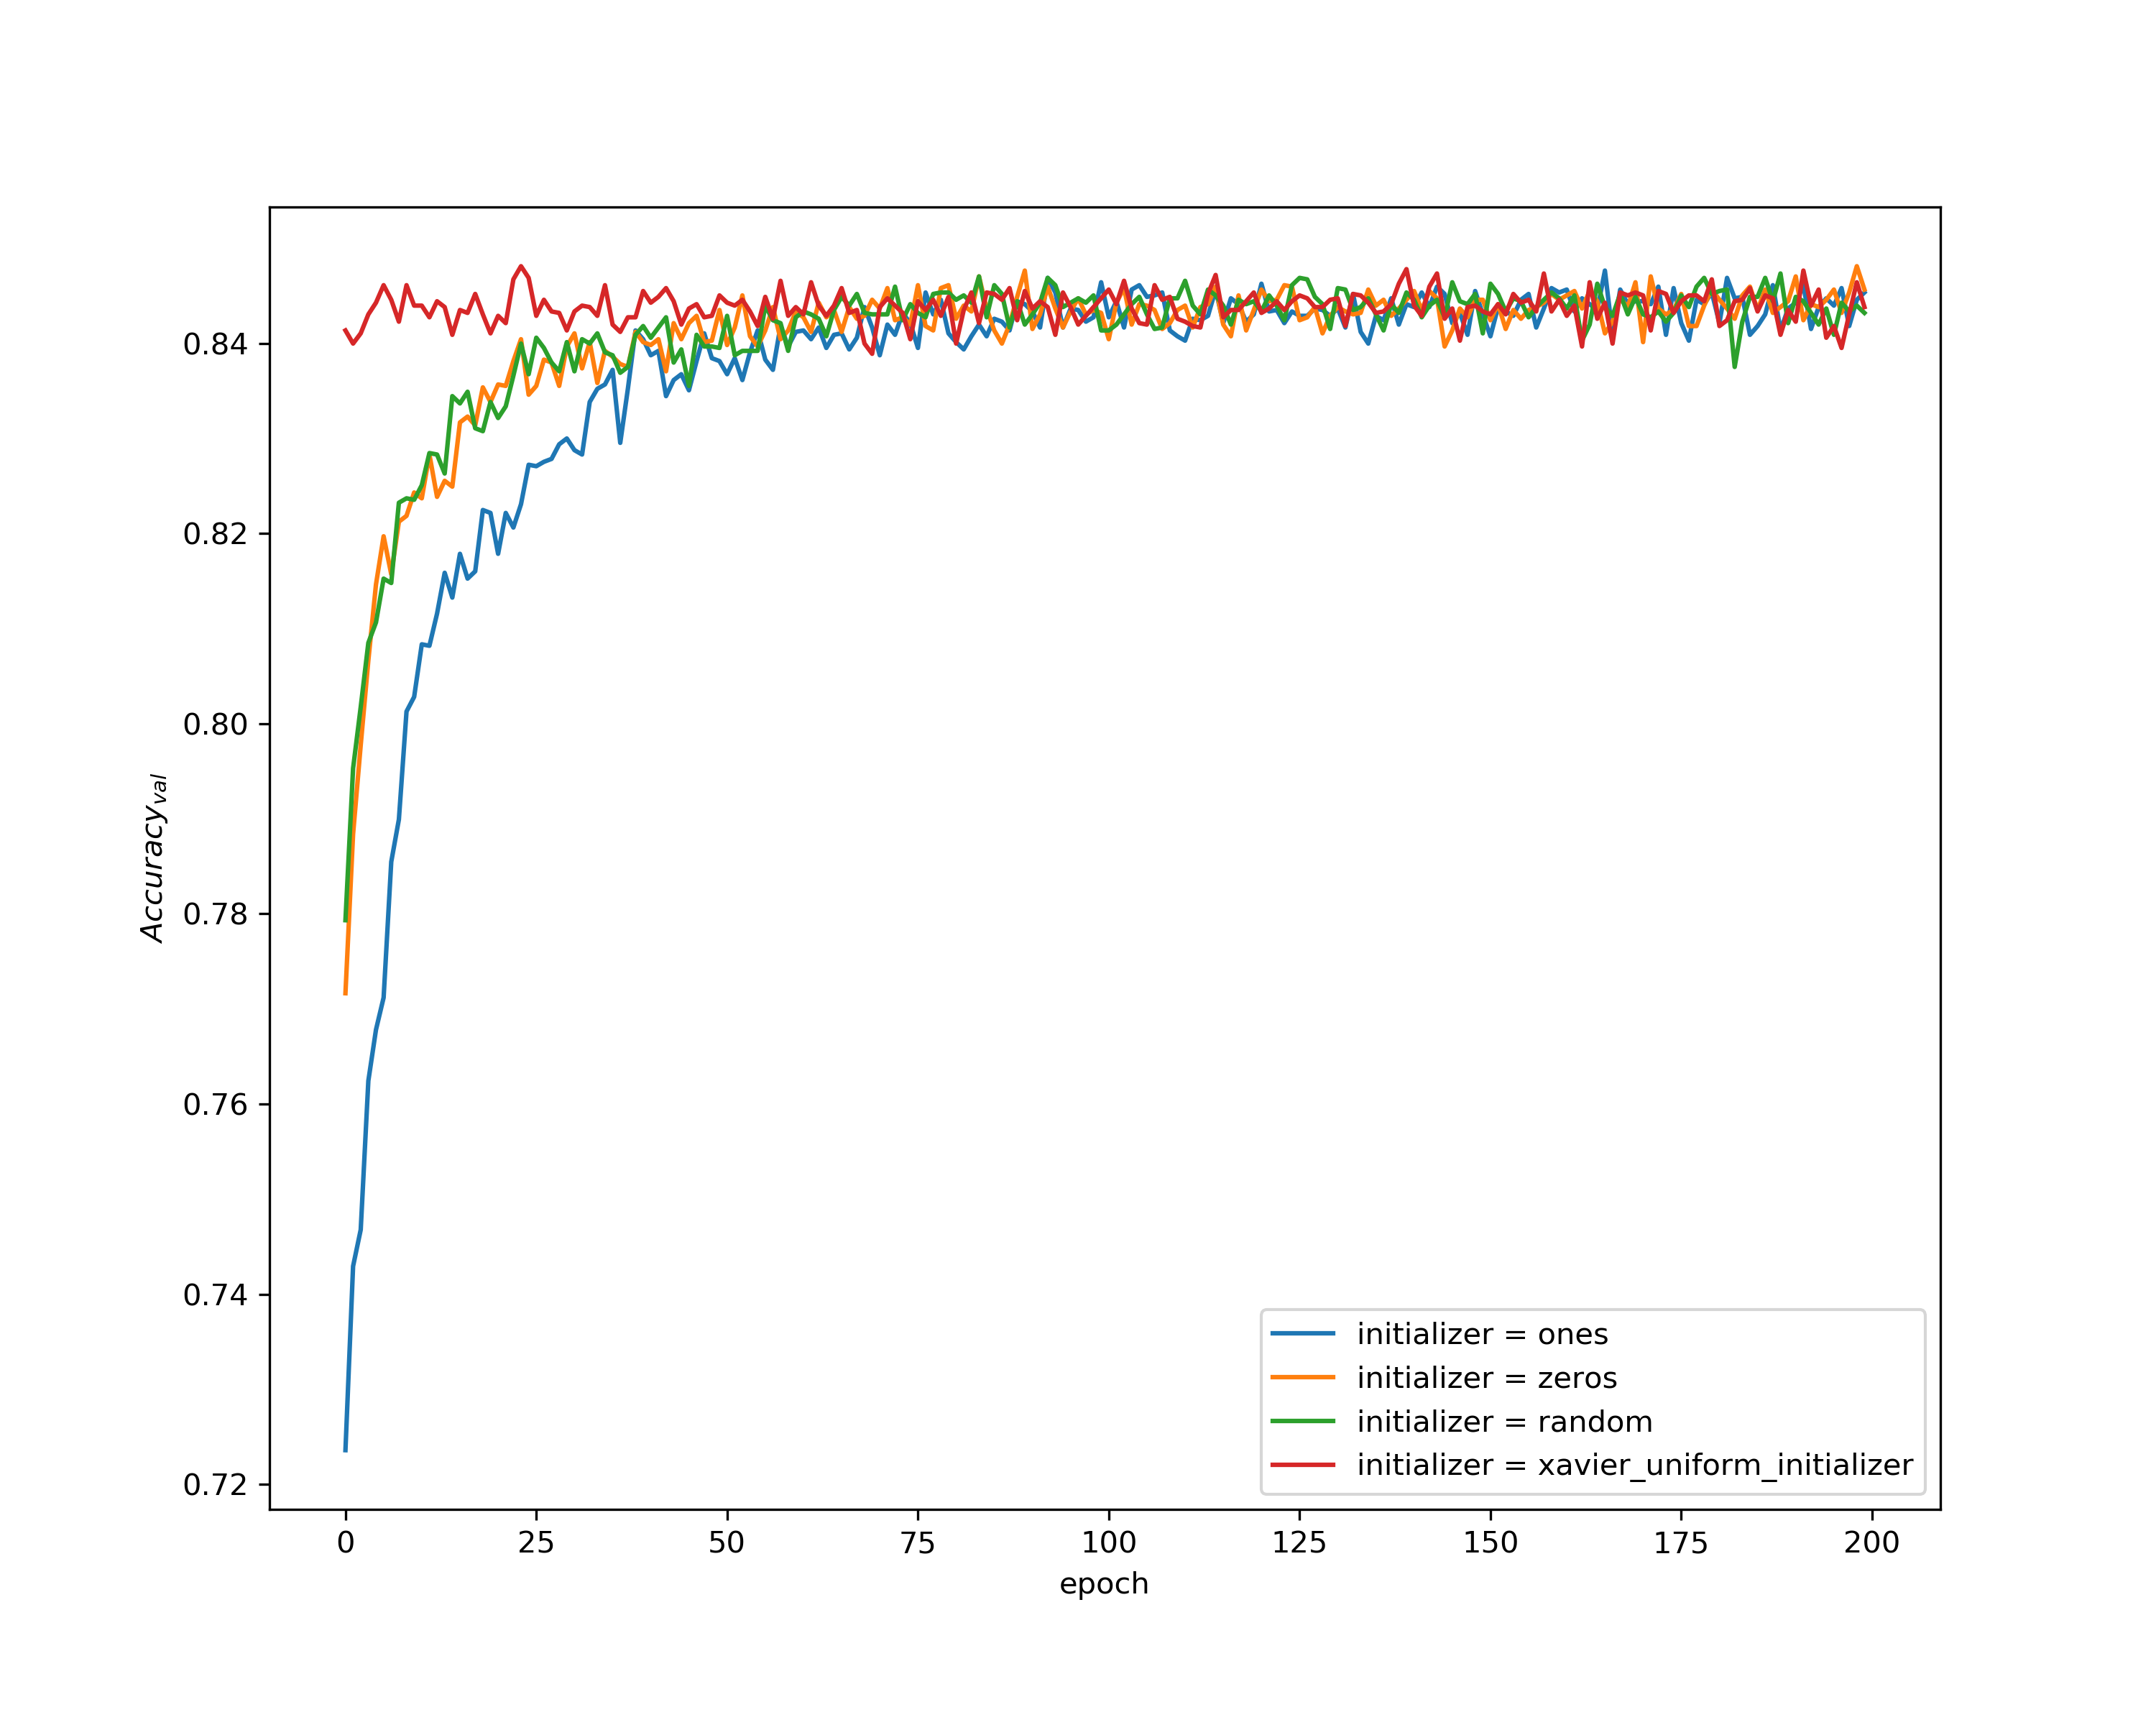
\includegraphics[width=\columnwidth]{svm_init_val_acc}
		% Create a subtitle for the figure.
		\caption{SVM's $Accuracy_{val}$ under different initilizer.}
		% Define the label of the figure. It's good to use 'fig:title', so you know that the label belongs to a figure.
		\label{fig:svm_init_val_acc}
	\end{center}
\end{figure} \par

\subsection{Optimizer comparision in both LR and SVM}
In this section, we compare the performance of LR and SVM with different optimizers. We explore over Stochastic Gradient Descent (SGD), Momentum, Adam and RMSProp. We use xavier uniform initializer, set learning rate to 0.001 epoch to 200, batch size to 64 and C to 10 in SVM. We use HL as SVM's loss function and BCE as LR's loss function.\par
From Fig~\ref{fig:lr_optim_val_loss} and Fig~\ref{fig:lr_optim_val_acc}, we can see that LR's performance is affected by the optimizer. Typically SGD converges very slowly; Momentum converges faster than SGD, but not as good as SGD's performance; both Adam and RMSProp converge very fast and get to the best performance.\par
From Fig~\ref{fig:svm_optim_val_loss} and Fig~\ref{fig:svm_optim_val_acc}, we can see that SVM is very robust to the optimizer too, different optimizer didn't disturb the performance except Momentum which converges slower and get worse performance comparing with other optimizers. \par

\begin{figure}[!hbt]
	% Center the figure.
	\begin{center}
		% Include the eps file, scale it such that it's width equals the column width. You can also put width=8cm for example...
		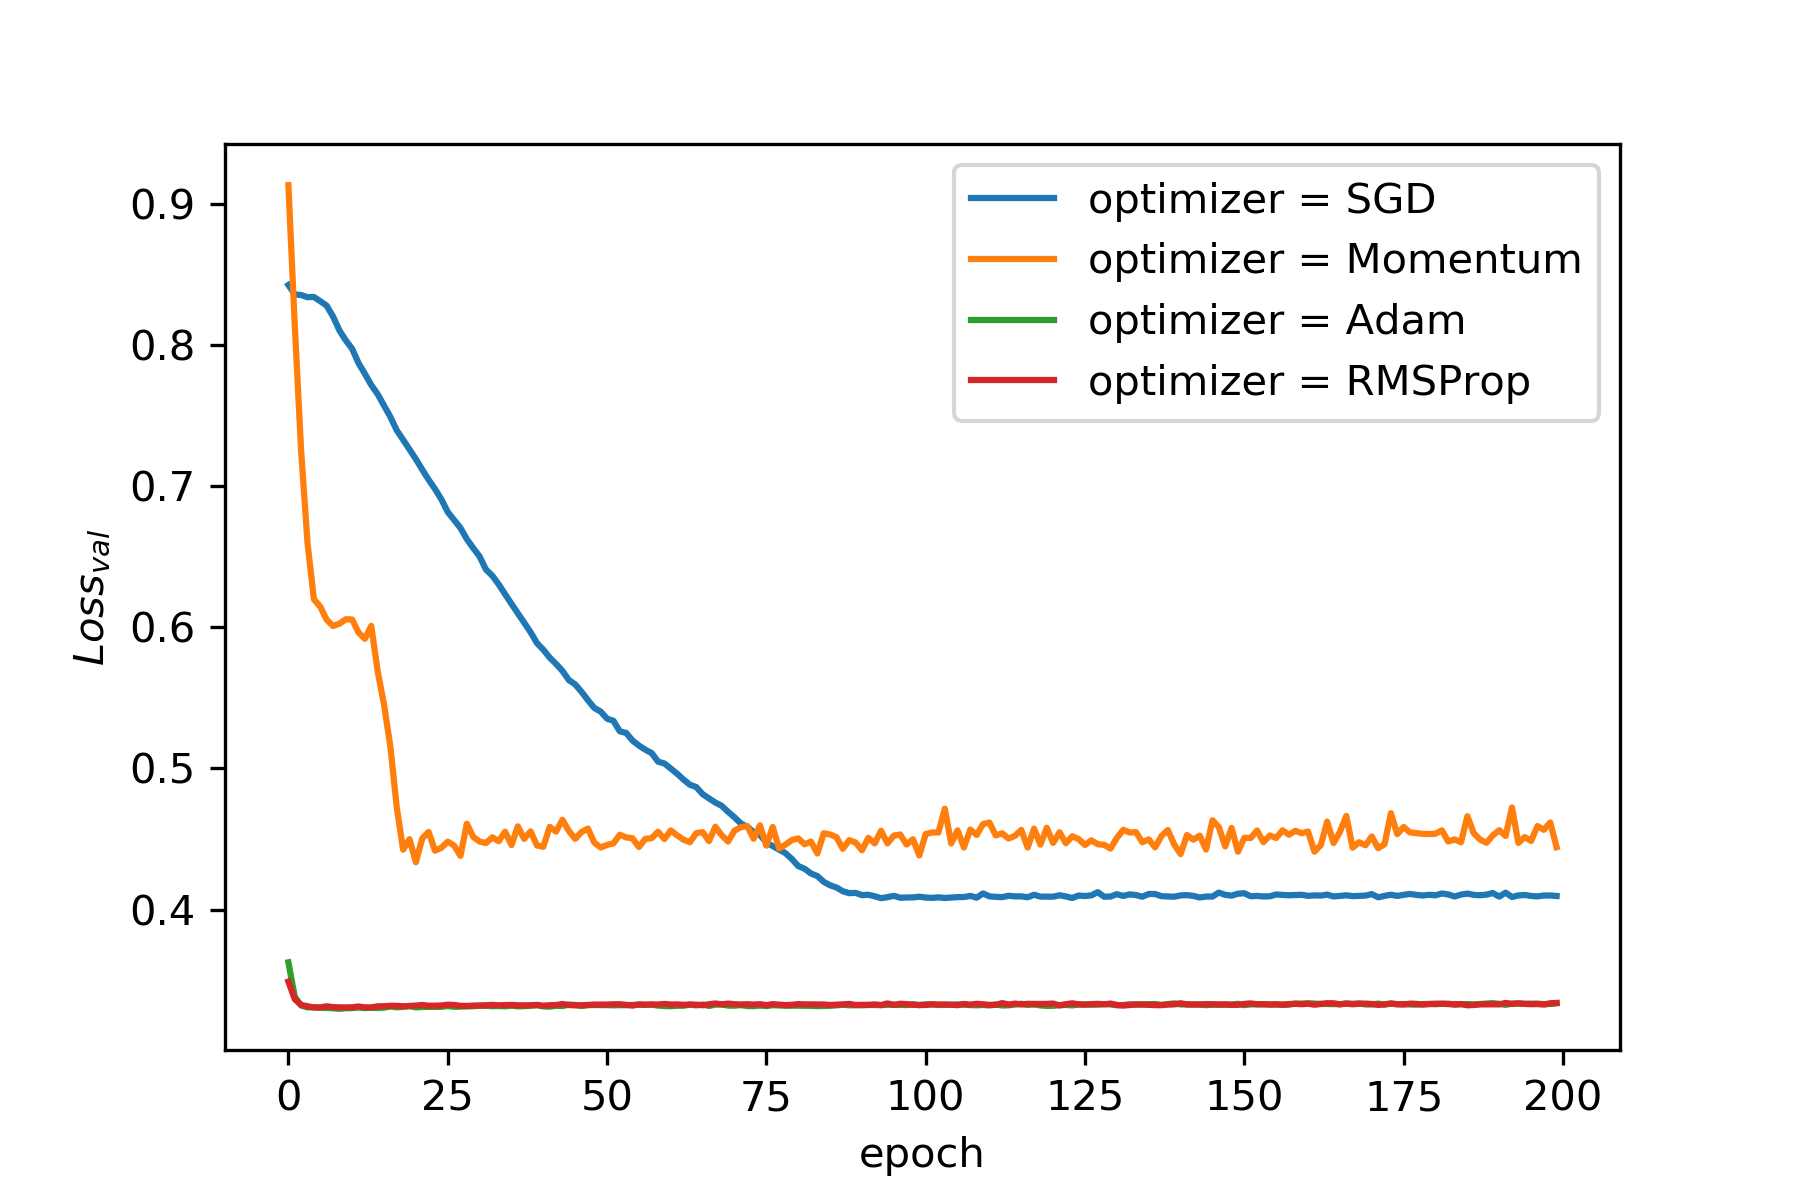
\includegraphics[width=\columnwidth]{lr_optim_val_loss}
		% Create a subtitle for the figure.
		\caption{LR's $BCE_{val}$ under different optimizer.}
		% Define the label of the figure. It's good to use 'fig:title', so you know that the label belongs to a figure.
		\label{fig:lr_optim_val_loss}
	\end{center}
\end{figure} \par

\begin{figure}[!hbt]
	% Center the figure.
	\begin{center}
		% Include the eps file, scale it such that it's width equals the column width. You can also put width=8cm for example...
		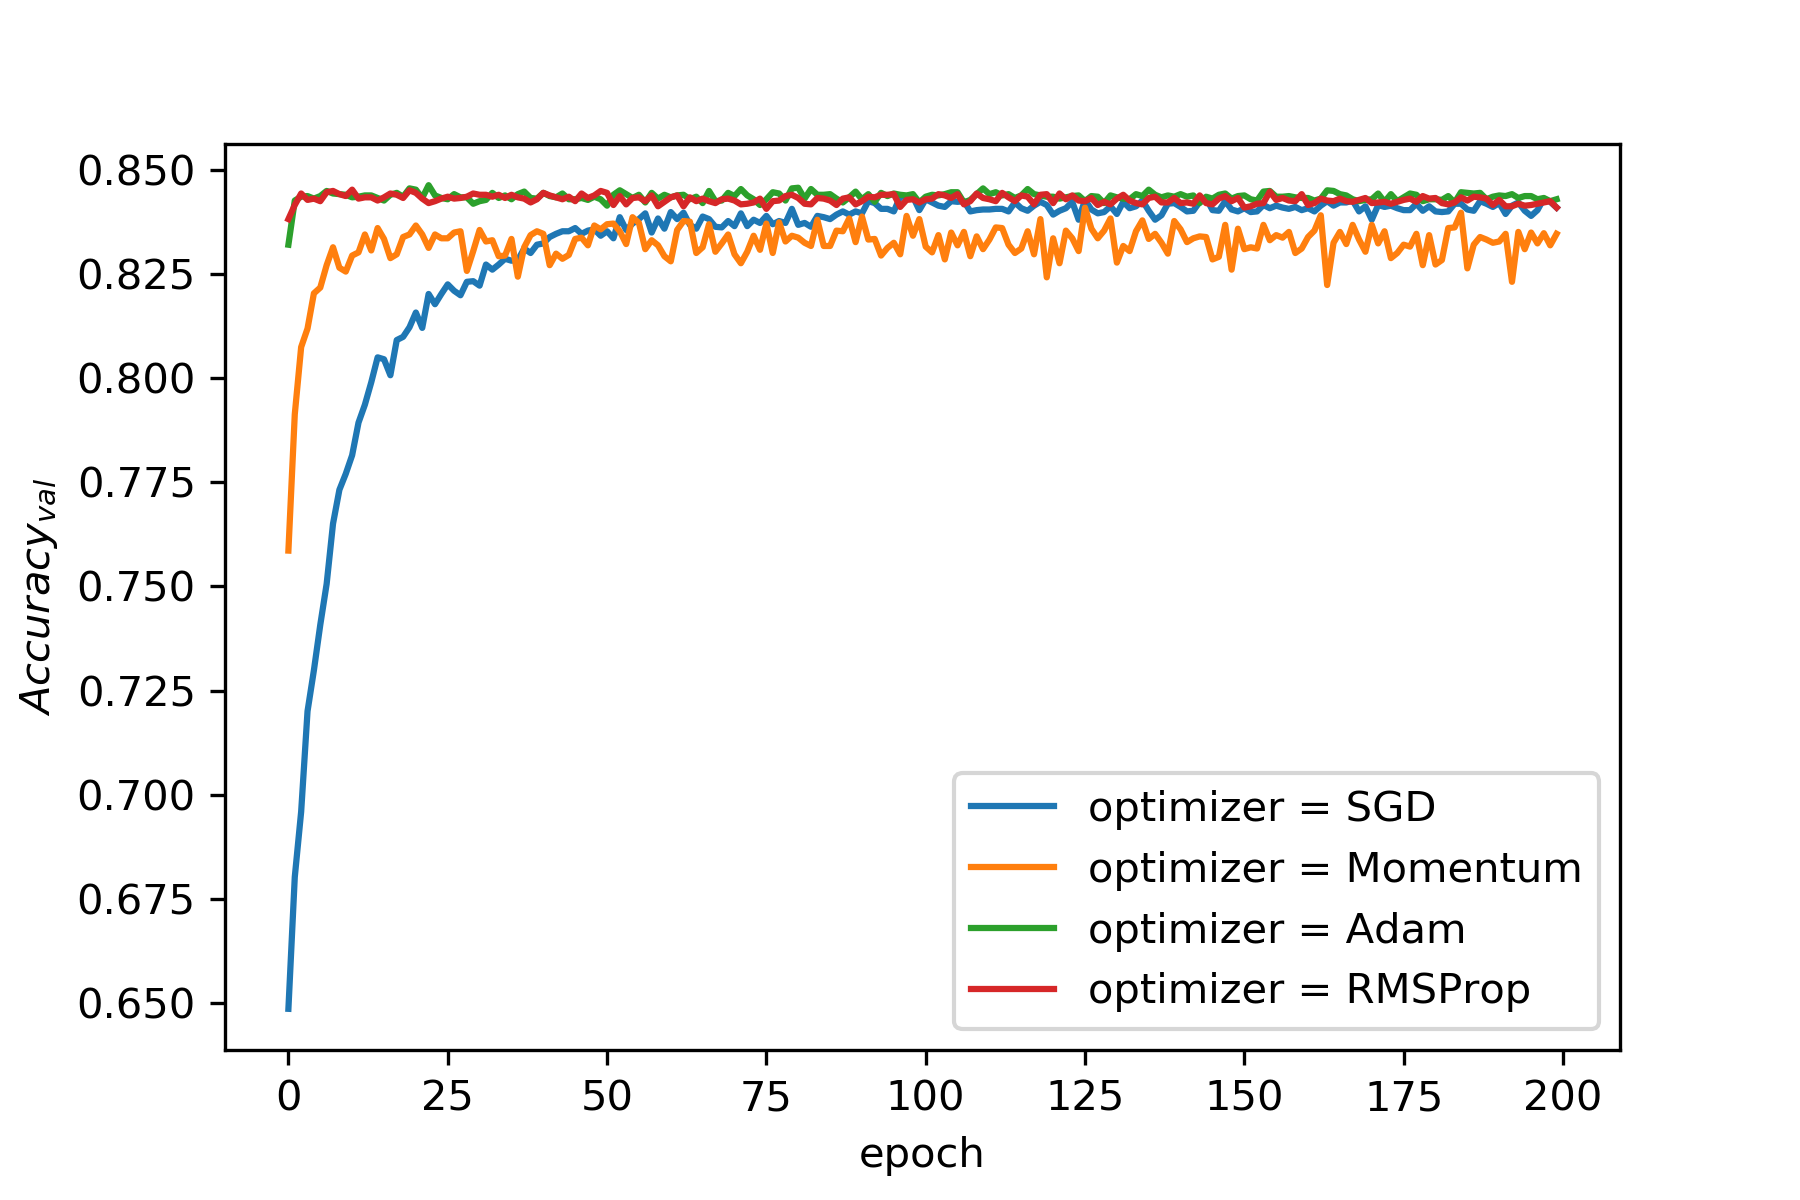
\includegraphics[width=\columnwidth]{lr_optim_val_acc}
		% Create a subtitle for the figure.
		\caption{LR's $Accuracy_{val}$ under different optimizer.}
		% Define the label of the figure. It's good to use 'fig:title', so you know that the label belongs to a figure.
		\label{fig:lr_optim_val_acc}
	\end{center}
\end{figure} \par

\begin{figure}[!hbt]
	% Center the figure.
	\begin{center}
		% Include the eps file, scale it such that it's width equals the column width. You can also put width=8cm for example...
		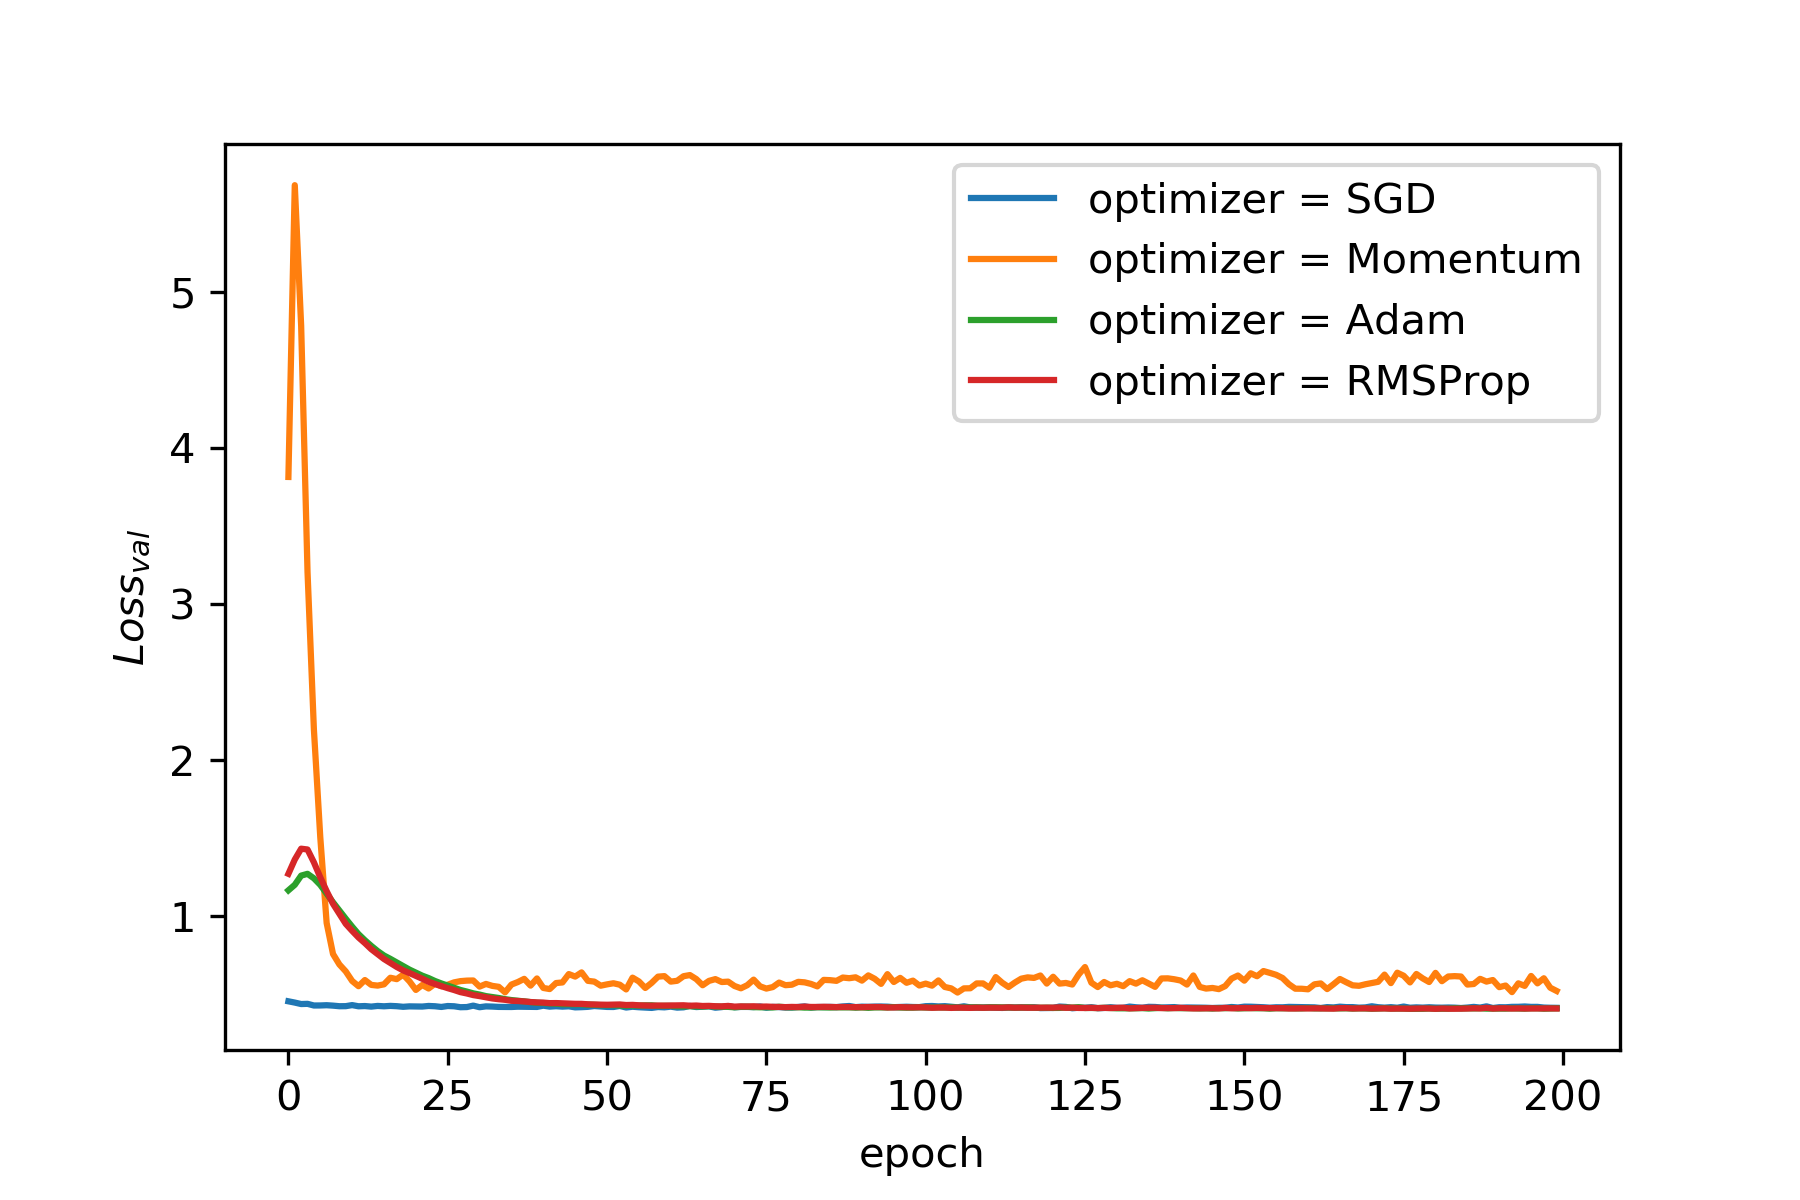
\includegraphics[width=\columnwidth]{svm_optim_val_loss}
		% Create a subtitle for the figure.
		\caption{SVM's $HL_{val}$ under different optimizer.}
		% Define the label of the figure. It's good to use 'fig:title', so you know that the label belongs to a figure.
		\label{fig:svm_optim_val_loss}
	\end{center}
\end{figure} \par

\begin{figure}[!hbt]
	% Center the figure.
	\begin{center}
		% Include the eps file, scale it such that it's width equals the column width. You can also put width=8cm for example...
		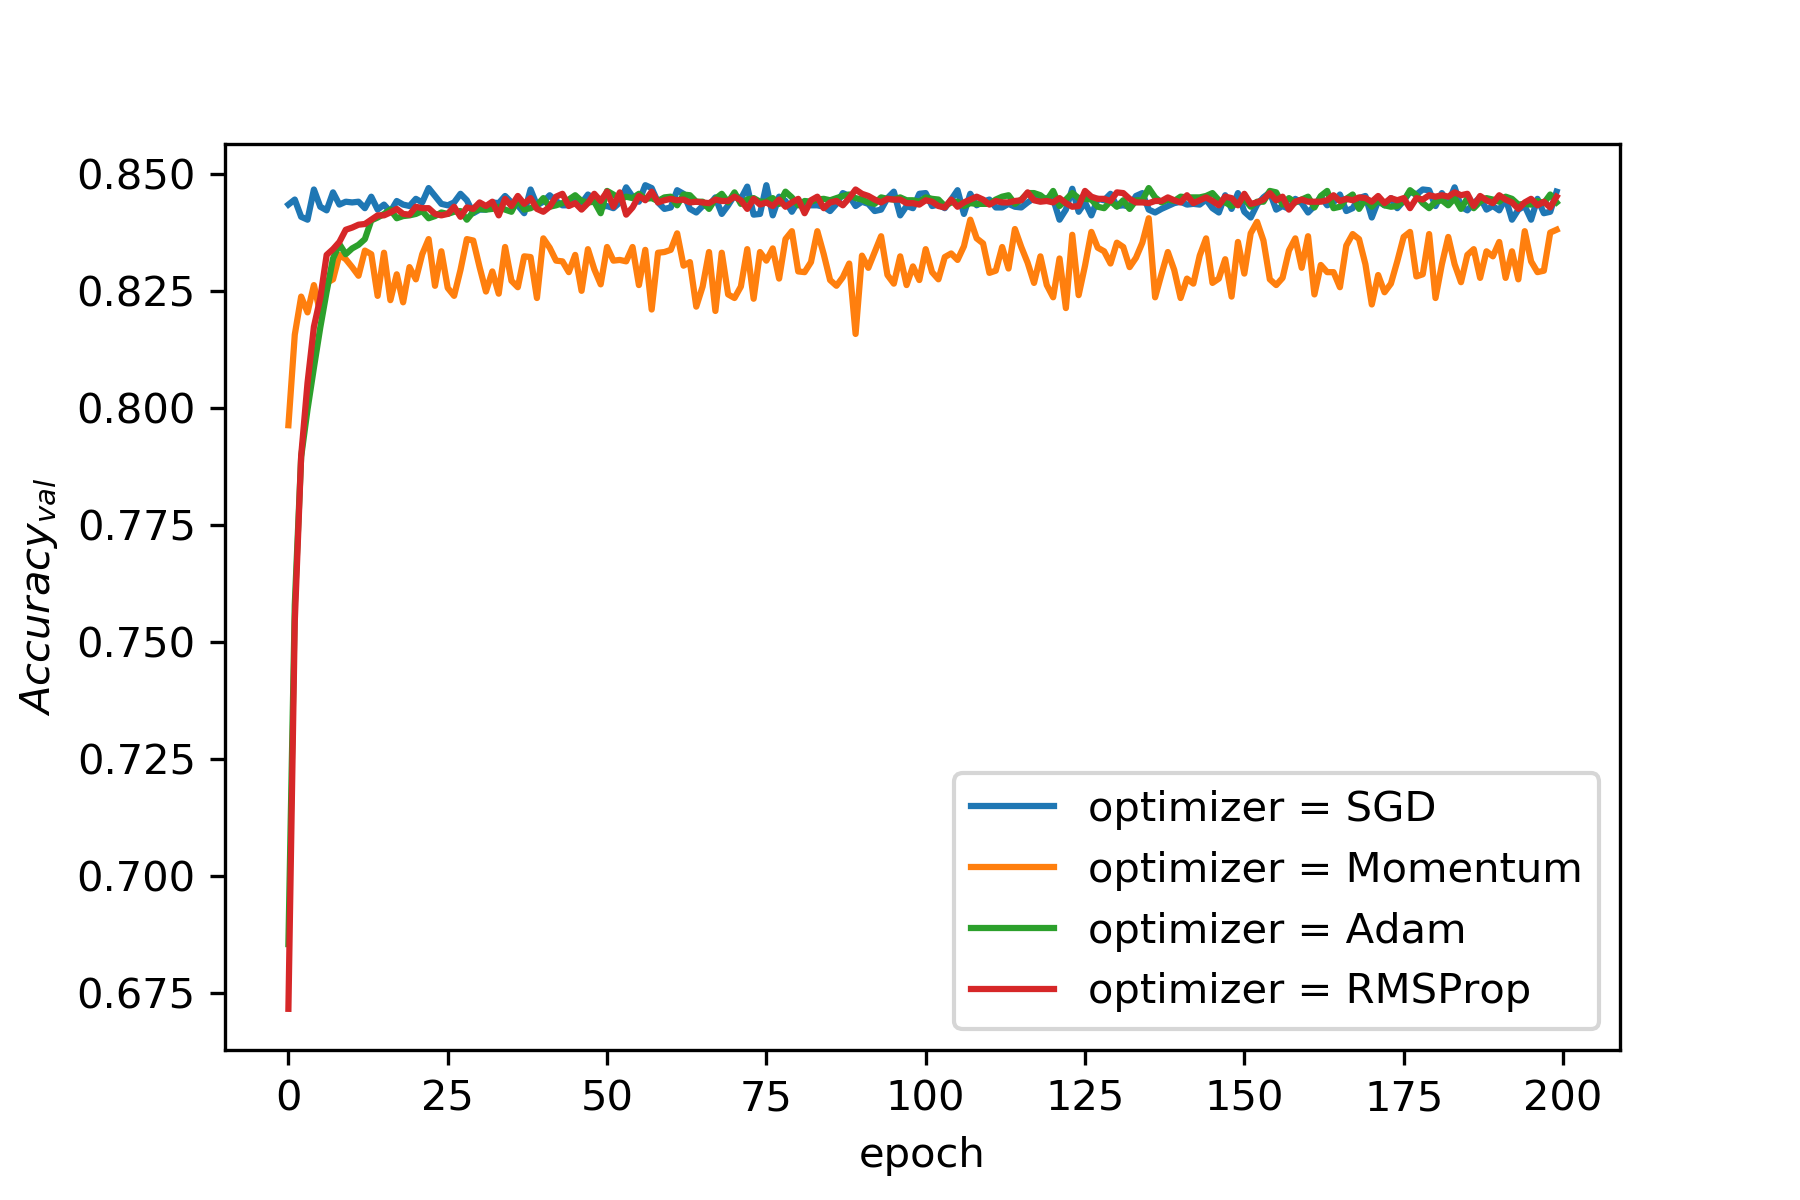
\includegraphics[width=\columnwidth]{svm_optim_val_acc}
		% Create a subtitle for the figure.
		\caption{SVM's $Accuracy_{val}$ under different optimizer.}
		% Define the label of the figure. It's good to use 'fig:title', so you know that the label belongs to a figure.
		\label{fig:svm_optim_val_acc}
	\end{center}
\end{figure} \par


\section{Conclusion}
In this report, we explore the CFS optimized LR, CFS optimized RR and MBGD optimized LR. We conduct the experiments on the CFS optimized LR and RR in terms of performance and weight magnitude. We also explore GD, SGD, MBGD in terms of convergence and time efficiency. Moreover, we tuning the hyper-parameter learning rate in MBGD. We also compare the weight magnitude between CFS optimized LR and MBGD optimized LR. Finally, we report the performance in CFS optimized LR, RR and MBGD LR. After a series of experiments, we now get more insight of LR, RR and GD and its variants SGD and MBGD. \par



% Your document ends here!


\end{document}